\chapter{Two-Flavor Quark-Meson Model}
\label{chap:lsm2f}

At low energy the effective degrees of freedom of quantum chromodynamics are not individual quarks,
but nucleons composed of up and down quarks and the three pions that we saw arose from the spontaneous chiral symmetry breaking pattern \eqref{eq:qcd:symmetry_breaking_pattern}.
The MIT bag model that we discussed in \cref{chap:mit} modeled quark stars as a deconfined Fermi gas of quarks with a bag constant $B$.
We will now crank up the difficulty and investigate the \textbf{linear sigma model}, which also takes chiral symmetry breaking and the pions into account by introducing an ``ad--hoc'' $\sigma$ particle.
The linear sigma model was originally introduced by \cite{ref:lsm_original} as an effective model for nucleons interacting with pions and scalar mesons,
but the fermions have since been interpreted as quarks in what is commonly referred to as a \textbf{quark-meson model}.

Quark stars consisting only of two-flavor quark matter are unlikely to be found in nature,
as two-flavor quark matter is observed to be unstable compared to hadronic matter.
Nevertheless, they are a natural stepping stone for modeling possibly stable strange quark stars
and dense hybrid neutron stars whose core could be made up of two-flavor quark matter.

The physical justification for this effective model of quantum chromodynamics is best made retrospectively after seeing exactly how it gives rise to chiral symmetry breaking.
We will therefore take the model as granted from the start and try to justify it as we go along.

\textit{This chapter is inspired by references \cite{ref:lsm_2f}, \cite{ref:lsm_notes} and \cite{ref:jo_lsm_consistent_physical}.}

\begin{figure}
\centering
\tikzsetnextfilename{potential}
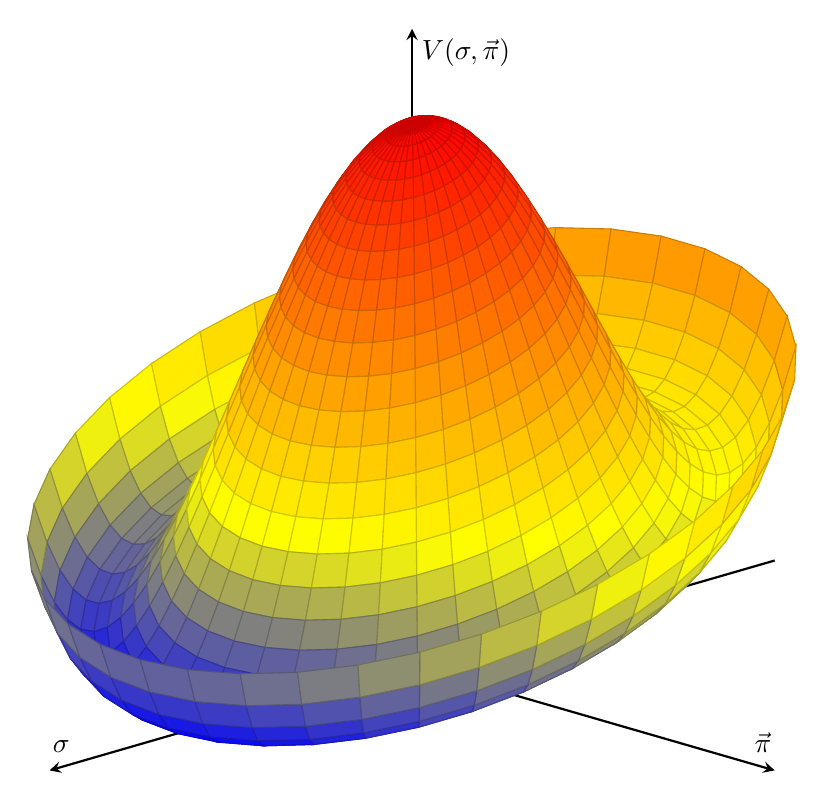
\begin{tikzpicture}
\begin{axis}[
	width = 20cm, height=15cm,
	%title = {Potential},
	xlabel = $\sigma$, ylabel = $\vec\pi$, zlabel = {$V(\sigma,\vec\pi)$},
	xmin=-4.0, xmax=+4.0, ymin=-4.0, ymax=+4.0, zmin=0, zmax=2.2,
	xtick=\empty, ytick=\empty, ztick=\empty,
	axis lines=center,
	axis line style = thick,
	view={135}{25},
	%colormap/blackwhite, mesh/interior colormap name=plasmarev,
]
	\addplot3 [surf, thin, domain=0:3.0, domain y=0:2*pi, samples=30, samples y=40, z buffer=sort] ({x*cos(deg(y))},{x*sin(deg(y))},{-1/2*((x*cos(deg(y)))^2+(x*sin(deg(y)))^2) + 1/24*((x*cos(deg(y)))^2+(x*sin(deg(y)))^2)^2 + 3/2 - 0.15*x*cos(deg(y)) + 0.15*sqrt(6)});
	%\addplot3 [domain=0:2*pi, samples=50, samples y=1] ({sqrt(6)*cos(deg(x))},{sqrt(6)*sin(deg(x))},{0});
\end{axis}
\end{tikzpicture}
\caption{\label{fig:lsm:potential}%
	A two-dimensional realization of the potential \eqref{eq:lsm:potential} looks like a Mexican hat, tilted along the $\sigma$-axis by the explicit symmetry breaking parameter $h$.
	If $h = 0$, the hat is upright with a continuous range of minima around $\sigma^2 + \vec\pi^2 = -6m^2 / \lambda$;
	while if $h \neq 0$, the hat is tilted and has a unique global minimum determined by equation \eqref{eq:lsm:ground_state_implicit}.
}
\end{figure}

\section{Lagrangian, symmetries and physical justification}
\label{sec:lsm:vacuum}

The Lagrangian density for the linear sigma model coupled to quarks is \cite{ref:lsm_2f}
\begin{equation}
	\lagr = \bar{q} \Big[ i \slashed\partial + \mu \gamma^0 - g \big( \sigma + i \gamma^5 \vec\tau \cdot \vec\pi \big) \Big] q
	      + \frac12 \Big[ \big( \partial_\mu \sigma \big) \big( \partial^\mu \sigma \big) + \big( \partial_\mu \vec\pi \big) \big( \partial^\mu \vec\pi \big) \Big] - \pot(\sigma,\vec\pi)
\label{eq:lsm:lagrangian}
\end{equation}
with the meson potential
\begin{equation}
	\pot(\sigma, \vec\pi) = \frac{m^2}{2} \big( \sigma^2 + \vec\pi^2 \big) + \frac{\lambda}{4!} \big( \sigma^2 + \vec\pi^2 \big)^2 - h \sigma .
\label{eq:lsm:potential}
\end{equation}
The quark fields behave as in the MIT bag model Lagrangian \eqref{eq:mit:lagrangian} with $N_f=2$ flavor indices $\{u,d\}$, $N_c=3$ color indices and four Dirac spinor indices, and are coupled to two quark chemical potentials with the flavor-space matrix $\mu = \diag (\mu_u, \mu_d)$.
However, they are now seemingly massless and coupled to a $\sigma$ meson and three pions $\vec\pi = [\pi^+, \pi^-, \pi^0]^T$ with a Yukawa coupling $g$ and the Pauli matrices \eqref{eq:tft:pauli_matrices}.
The meson potential features three couplings $m^2<0$, $\lambda>0$ and $h>0$.

Like quantum chromodynamics, the quark-meson model Lagrangian \eqref{eq:lsm:lagrangian} has a vector $U(1)_V$ and an axial $U(1)_A$ symmetry shown in \cref{sec:master_intro:qcd}.
In contrast to the mass-conditional chiral symmetry of quantum chromodynamics, however,
the Lagrangian \eqref{eq:lsm:lagrangian} is \emph{unconditionally} invariant under a $SU(2)_L \times SU(2)_R$ transformation when $h=0$ and $\mu = 0$.
To see this, first express the Yukawa coupling term with left-handed and right-handed chiral fields $q_\pm = P_\pm q$:
\begin{equation}
\begin{aligned}
	\bar{q} \big[\sigma + i \gamma^5 \vec{\tau} \cdot \vec{\pi}\big] q &= \bar{q} \big[ (P_+ + P_-) \sigma + (P_+ - P_-) i \vec{\tau} \cdot \vec{\pi}\big] q && \; \big( P_\pm = \tfrac{1}{2} (1 \pm \gamma^5) \big) \\
	                                                           %&= \bar{q} \big[ P_+ (\sigma + i \vec{\tau} \cdot \vec{\pi}) + P_- (\sigma - i \vec{\tau} \cdot \vec{\pi}) \big] q && \; \big( \text{distributivity} \big)\\
	                                                           &= \bar{q} \big[ P_+ \phi + P_- \phi^\dagger\big] q && \; \big( \text{define } \phi=\sigma+i\vec{\tau}\cdot\vec{\pi} \big) \\
	                                                           &= \bar{q} \big[ P_+^2 \phi + P_-^2 \phi^\dagger\big] q && \; \big( \text{$P_\pm=P_\pm^2$ lives in spinor-space} \big) \\
	                                                           &= \bar{q} \big[ P_+ \phi P_+ + P_- \phi^\dagger P_-\big] q && \; \big( \text{$\phi$ lives in flavor-space} \big)\\
	                                                           &= \bar{q}_- \phi \, q_+ + \bar{q}_+ \phi^\dagger q_- && \; \big( \text{$P_\pm q = q_\pm$, $\bar{q} P_\pm = (P_\mp q)^\dagger \gamma^0 = \bar{q}_\mp$} \big).\\
\end{aligned}
\label{eq:lsm:yukawa_symmetry}
\end{equation}
Second, note that the meson potential \eqref{eq:lsm:potential} with $h=0$ only depends on the flavor-space trace
\begin{equation}
	\tfrac12 \trace\big[\phi^\dagger \phi\big] = \tfrac12 \big( \underbrace{\trace\big[1\big]}_2 \sigma^2 - i^2 \underbrace{\trace\big[\tau_a \tau_b \big]}_{2 \delta_{ab}} \pi_a \pi_b \big) = \sigma^2 + \vec{\pi}^2.
\label{eq:lsm:meson_symmetry}
\end{equation}
Under the $SU(2)_L \times SU(2)_R$ transformation 
\begin{equation}
	q_+ \rightarrow U_+ q_+, \qquad
	q_- \rightarrow U_- q_-
	\qquad \text{and} \qquad
	\phi   \rightarrow U_- \phi U_+^\dagger,
\label{eq:lsm:symmetry_transformation}
\end{equation}
the Yukawa interaction \eqref{eq:lsm:yukawa_symmetry},
the meson potential argument \eqref{eq:lsm:meson_symmetry}
and hence the Lagrangian \eqref{eq:lsm:lagrangian} are invariant.
This proves the claimed unconditional $SU(2)_L \times SU(2)_R$ symmetry when $h=0$ and $\mu=0$.
Since the group $SU(2)_L \times SU(2)_R$ is isomorphic to $O(4)$,
the symmetry can equivalently be understood by considering the meson fields as a four-vector $[\sigma, \vec{\pi}]^T$
and noting that the meson potential \eqref{eq:lsm:potential} is invariant under rotation of this vector in four-space.

What can be the relevance of this unconditional symmetry,
when it was precisely the \emph{breaking} of it that led to the chiral symmetry breaking \eqref{eq:qcd:symmetry_breaking_pattern} of quantum chromodynamics in \cref{sec:master_intro:qcd}?
The short answer is that at the end of the day,
the different mathematical symmetries give rise to the \emph{same} physical consequences.
The longer answer follows below.

In the vacuum, the fermions do not contribute to the grand potential,
and the ground state values $\sigma = \avg{\sigma}$ and $\vec{\pi} = \avg{\vec{\pi}}$
are given by minima of the meson potential $\pot(\avg{\sigma},\avg{\vec{\pi}})$ illustrated in \cref{fig:lsm:potential}.
From its definition \eqref{eq:lsm:potential},
we see that they are given by
\begin{equation}
	%\vec{\pi} = \avg{\vec{\pi}}
	%\quad \text{and} \quad
	%\sigma = \avg{\sigma}
	%\pdv{\pot}{\sigma}_{(\sigma,\vec\pi)=(\avg{\sigma},\vec{0})} = m^2 \avg{\sigma} + \frac{\lambda}{6} \avg{\sigma}^3 - h = 0.
	\pdv{\pot}{\pi_a} = \avg{\pi_a} \Big[ m^2 + \frac{\lambda}{6} \big(\avg{\sigma}^2 + \avg{\vec{\pi}}^2\big) \Big] = 0
	\quad \text{and} \quad
	\pdv{\pot}{\sigma} = \avg{\sigma} \Big[ m^2 + \frac{\lambda}{6} \big(\avg{\sigma}^2 + \avg{\vec{\pi}}^2\big) \Big] - h = 0.
\label{eq:lsm:ground_state_implicit}
\end{equation}
The qualitative nature of the solutions depend on whether $h$ vanishes:
\begin{itemize}
\item In the \textbf{chiral limit} $h=0$,
      the ground state solutions are a degenerate range of minima along the circle $\avg{\sigma}^2+\avg{\vec{\pi}}^2=-6m^2/\lambda$,
      sometimes referred to as a vacuum manifold.
      Without any loss of generality, we pick the one at $\avg{\sigma} = \sqrt{-6m^2/\lambda}>0$ and $\avg{\vec{\pi}}=0$.
\item At the \textbf{physical point} $h \neq 0$,
      the ground state of the potential is a unique global minimum at $\avg{\sigma} \neq 0$ and $\avg{\vec{\pi}}=0$ determined implicitly by equation \eqref{eq:lsm:ground_state_implicit}.
\end{itemize}
Note that $\avg{\vec{\pi}} = 0$ in both cases.
To account for quantum fluctuations $\tilde{\sigma}$ and $\tilde{\vec{\pi}}$ of $\sigma$ and $\vec{\pi}$ around the ground states $\avg{\sigma}$ and $\avg{\vec{\pi}}$,
let us write
\begin{equation}
	\sigma = \avg{\sigma} + \tilde{\sigma}
	\qquad \text{and} \qquad
	\vec\pi = \avg{\vec\pi} + \tilde{\vec{\pi}}.
\end{equation}
Up to second order in the quantum fluctuations,
the Lagrangian \eqref{eq:lsm:lagrangian} becomes
\begin{equation}
	\lagr = \sum_{f=1}^{\smash{N_f}} \sum_{c=1}^{N_c} \bar{q} \Big[ i \slashed\partial + \mu \gamma^0 - m_q \Big] q
	      + \frac12 \Big[ \big( \partial_\mu \tilde{\sigma} \big) \big( \partial^\mu \tilde{\sigma} \big) + \big( \partial_\mu \tilde{\vec\pi} \big) \big( \partial^\mu \tilde{\vec\pi} \big) \Big] - \pot(\sigma,\vec\pi) , %\pot(\avg{\sigma}+\tilde{\sigma},\avg{\vec\pi}+\tilde{\vec\pi}) ,
\end{equation}
with the second-order meson potential \eqref{eq:lsm:potential}
\begin{equation}
	\pot(\sigma,\vec\pi) = \pot(\avg{\sigma},\avg{\vec\pi}) + h \tilde{\sigma} + \frac12 m_\sigma^2 \tilde{\sigma}^2 + \frac12 m_\pi^2 \tilde{\pi}^2,
\end{equation}
where the quark and meson fields have acquired the effective masses
\begin{subequations}
\begin{align}
	m_q &= g \avg{\sigma}, \label{eq:lsm:mass_quark} \\
	m_\sigma^2 &= \pdv[2]{\pot}{\sigma}\iffalse_{\substack{\sigma=\avg{\sigma}\\\vec{\pi}=\avg{\vec{\pi}}}}\fi    = m^2 + \frac{\lambda}{2} \avg{\sigma}^2 \equalexplabove{\smash[t]{\text{ by \eqref{eq:lsm:ground_state_implicit}}}} \frac{3h}{\avg{\sigma}} - 2 m^2 , \label{eq:lsm:mass_sigma} \\
	m_\pi^2    &= \pdv[2]{\pot}{\vec{\pi}}\iffalse_{\substack{\sigma=\avg{\sigma}\\\vec{\pi}=\avg{\vec{\pi}}}}\fi = m^2 + \frac{\lambda}{6} \avg{\sigma}^2 \equalexplbelow{\smash[b]{\text{ by \eqref{eq:lsm:ground_state_implicit}}}} \frac{h}{\avg{\sigma}} . \label{eq:lsm:mass_pi}
\end{align}%
\label{eq:lsm:mass_sigmapi}%
\end{subequations}%

Note that the up and down quarks have a degenerate mass $m_u = m_d = m_q$.
In nature, isospin symmetry is seemingly only slightly broken, and the up and down quark masses are indeed almost equal.
The squared meson masses $m_\sigma^2$ and $m_\pi^2$ are called \emph{curvature masses}
due to their relation with the second derivative of the potential.
They coincide with the physical pole masses of the particles' propagators
only at tree level, where loop effects are neglected.
\TODO{ok?}

The qualitative nature of the pions depends on whether $h$ vanishes:
\begin{itemize}
\item In the \textbf{chiral limit} $h = 0$ the $SU(2)_L \times SU(2)_R$ symmetry \eqref{eq:lsm:symmetry_transformation} is exact,
      and we saw above that there is a vacuum manifold of ground states.
      Upon committing to the minimum above with $\avg{\sigma} \neq 0$ and $\avg{\vec{\pi}} = 0$, the $O(4)$ rotation symmetry of the four original meson fields $[\sigma,\vec\pi]^T$ is spontaneously broken
      to rotation of only the three pion quantum fluctuations $\tilde{\vec\pi}$ in $O(3)$.
      Accordingly, the pion mass \eqref{eq:lsm:mass_pi} vanishes and the three pions are indeed Goldstone bosons associated with spontaneous symmetry breaking.
\item At the \textbf{physical point} $h \neq 0$, the $SU(2)_L \times SU(2)_R$ symmetry \eqref{eq:lsm:meson_symmetry} is explicitly broken,
      and we saw above that there is a unique ground state.
      Accordingly, the pions gain small masses \eqref{eq:lsm:mass_pi} and are pseudo-Goldstone bosons.
\end{itemize}
\label{elaborate on mexican hat analogy, brim, tip/tilt, etc.}
Unlike the resulting pions, the $\sigma$ particle is the \emph{cause} of the symmetry breaking,
and there is no reason for its mass \eqref{eq:lsm:mass_sigma} to vanish.
Speaking brutally to make a point, the $\sigma$ meson is only a mere means to an end to generate the chiral symmetry breaking and three pions,
which are our favorite spoiled children in this group of four meson siblings.

To summarize: although the linear sigma model symmetry breaking pattern
\begin{equation}
	SU(2) \times SU(2) \simeq O(4) \qquad \longrightarrow \qquad O(3)
\end{equation}
is \emph{different} from the quantum chromodynamics symmetry breaking pattern \eqref{eq:qcd:symmetry_breaking_pattern} ``under the hood'',
it gives rise to exactly the \emph{same} pion degrees of freedom ``on the outside''.
Practically speaking, the two different symmetry breaking patterns are therefore indistinguishable,
and according to Weinberg's philosophy presented in \cref{sec:master_intro:qcd}
the quark-meson model is an appropriate effective model of quantum chromodynamics at low energy.
The parameter $h \neq 0$ only serves to explicitly break the symmetry into an approximate one,
just like the quark masses explicitly break the chiral symmetry of quantum chromodynamics.
This is the physical justification of the quark-meson model.

\section{Grand potential}
\label{sec:lsm:grand_potential}

With our recently gained faith in the quark-meson model,
we set out to calculate its grand potential \eqref{eq:master_intro:grand_potential}.
With the quark fields $q$, the meson fields $\sigma$ and $\vec\pi$
and the coupling of conserved currents $j^\mu = \bar{q} \gamma^\mu q$ to chemical potentials $\mu$ already baked into the Lagrangian \eqref{eq:lsm:lagrangian},
the partition function \eqref{eq:master_intro:partition_function} is
\begin{equation}
	Z = \oint_- \pathintdif \bar{q} \oint_- \pathintdif q \oint_+ \pathintdif \sigma \oint_+ \pathintdif \vec\pi \exp \left\{ \int_0^\beta \dif \tau \int_V \dif^3 x \, \lagr_E[\bar{q}, q, \sigma, \vec\pi]  \right\} .
\end{equation}
To calculate it we will use the \textbf{mean-field approximation} for the bosonic fields,
replacing them by their \emph{yet unknown} expectation values $\avg{\sigma}$ and $\avg{\vec\pi}$ in the classical ground state
and simply ignoring their quantum fluctuations $\tilde{\sigma}$ and $\tilde{\vec\pi}$.
In contrast we will give the fermions full treatment,
motivated by their more dramatic behavior at zero temperature.
After calculating the grand potential with unknown mean fields,
their precise values are found \emph{self-consistently} with the original assumption of them being minima of the grand potential by solving
\begin{equation}
	\pdv{\Omega}{\avg{\sigma}} = \pdv{\Omega}{\avg{\vec\pi}} = 0.
\label{eq:lsm:gap_equation}
\end{equation}
We call this the \textbf{self-consistency equation} for the mean fields.
For example, the mean-field approximation is also famously used in the Bardeen-Cooper-Schrieffer theory of superconductivity to determine an energy gap.
There it is called the \textbf{gap equation}, 
and it can be useful to know that this name lives on as a relic in completely different applications, too.

In our treatment we will also neglect pion condensation and assume that $\avg{\vec\pi}=0$ \emph{always} vanishes,
so that only $\avg{\sigma}$ needs to be determined.
As shown by \cite{ref:jo_lsm_pion_condensation,ref:jo_lsm_consistent}, for example,
this is known to be true at $T=0$ when the isospin chemical potential \eqref{eq:master_intro:chemical_potentials_transformed} does not exceed half the pion mass.
This assumption is subject to a self-consistency check later.
In the bosonic mean-field approximation, the partition function of the Lagrangian \eqref{eq:lsm:lagrangian} reads
\begin{equation}
	Z = \oint_- \pathintdif \bar{q} \oint_- \pathintdif q \exp \bigg\{ \int_0^{\beta} \dif \tau \! \int_V \dif^3 x \Big[ \bar{q} \big( i \slashed\partial - m_q + \mu_f \gamma^0 \big) q - \pot(\avg{\sigma},\vec{0}) \Big] \bigg\}.
\end{equation}
The meson potential is independent of the fields and can be pulled out of the integrals,
while the fermionic contribution decouples into a product of identical integrals.
We therefore have
\begin{equation}
\begin{split}
	%\log Z &= -\frac12 \beta V m^2 \avg{\sigma}^2 - \frac{\lambda}{4!} \beta V \avg{\sigma}^4 + \beta V h \avg{\sigma} \\
	       %&+ \sum_{f=1}^{N_f} \sum_{c=1}^{N_c} \log \oint_- \pathintdif \bar{q}_f^c \oint_- \pathintdif q_f^c \exp \left\{ \int_0^\beta \dif \tau \int_V \dif^3 x \, \bar{q}_f^c (i \slashed\partial + \mu_f \gamma^0 - m_q) q_f^c \right\} .
	\log Z = -\pot(\avg{\sigma},\vec{0}) + \sum_{f=1}^{\smash{N_f}} \sum_{c=1}^{N_c} \log \oint_- \!\! \pathintdif \bar{q}_{f,c} \oint_- \!\! \pathintdif q_{f,c} \exp \bigg\{ \! \int_0^\beta \! \dif \tau \int_V \! \dif^3 x \, \bar{q}_{f,c} \big(i \slashed\partial + \mu_f \gamma^0 - m_q\big) q_{f,c} \! \bigg\} .
\end{split}
\end{equation}
We have already calculated the path integral in the last term
from equation \eqref{eq:tft:dirac_partition_function_first} to equation \eqref{eq:tft:dirac_partition_function}.
Here we get a factor $\sum_{c=1}^{N_c} = N_c$ from the color sum because the summand is independent of $c$,
while the flavor sum $\sum_{f=1}^{\smash{N_f}}$ yields $N_f$ terms that differ only by the chemical potential $\mu_f$ associated with each quark flavor. 
Thus, the grand potential \eqref{eq:master_intro:grand_potential} is
\begin{equation}
\begin{split}
	%\log Z &= -\frac12 \beta V m^2 \avg{\sigma}^2 - \frac{\lambda}{4!} \beta V \avg{\sigma}^4 + \beta V h \avg{\sigma} \\
	       %&+ 2 V N_c \sum_{f=1}^{N_f} \int \frac{\dif^3 p}{(2 \pi)^3} \left\{ \beta E(\vec{p}) + \log \left[ e^{-\beta (E(\vec{p}) - \mu_f)}+1 \right] + \log \left[ e^{-\beta (E(\vec{p}) + \mu_f)} + 1\right] \right\} ,
	\Omega = \pot(\avg{\sigma},\vec{0}) - \frac{2 N_c}{\beta} \sum_{f=1}^{\smash{N_f}} \int \frac{\dif^3 p}{(2 \pi)^3} \left\{ \beta E(\vec{p}) + \log \left[ e^{-\beta (E(\vec{p}) - \mu_f)}+1 \right] + \log \left[ e^{-\beta (E(\vec{p}) + \mu_f)} + 1\right] \right\} ,
\end{split}
\label{eq:lsm:potential_divergent_logz0}
\end{equation}
with the dispersion relation $E(\vec{p}) = \sqrt{\smash[b]{p^2 + m_q^2}}$.
We work in the zero-temperature approximation $T=0$ and choose positive chemical potentials,
so the anti-particle contribution from the last term in curly brackets vanishes.
The integral of the middle term in curly brackets was calculated in the zero-temperature pressure $P=-\Omega$ in equation \eqref{eq:nstars:pressure_zeroT}.
This time we also include and renormalize the infinite vacuum contribution from the integral of the first term in curly brackets.
It is called the \emph{Dirac sea}, and we renormalize it in the modified minimal subtraction scheme in \cref{chap:diracsea}.
Reinstating $x_f = p_f / m_q = \sqrt{\smash[b]{\mu_f^2-m_q^2}} / m_q$ into expression \eqref{eq:nstars:pressure_zeroT}
and including the renormalized Dirac sea \eqref{eq:diracsea:pole_expansion_modified},
the divergent grand potential \eqref{eq:lsm:potential_divergent_logz0} becomes
\begin{equation}
\begin{split}
	\Omega &= \pot(\avg{\sigma},\vec{0}) + N_c N_f \frac{m_q^4}{16 \pi^2} \Bigg[ \textcolor{red}{\frac{1}{\epsilon}} + \frac{3}{2} + \log\left(\frac{{\Lambda}^2}{m_q^2}\right) \Bigg] \\
	       &- \sum_{f=1}^{\smash{N_f}} \frac{N_c}{24 \pi^2} \left[ \left( 2 \mu_f^2 - 5 m_q^2 \right) \mu_f \sqrt{\mu_f^2 - m_q^2} + 3 m_q^4 \asinh \left( \sqrt{\frac{\mu_{\smash{f}}^2}{m_q^2}-1} \right) \right] .
\end{split}
\label{eq:lsm:grand_potential_nonrenormalized}
\end{equation}
The renormalization has introduced a renormalization scale $\Lambda$ that we will determine later.
It also exposes the Dirac sea vacuum divergence in the $\epsilon$-pole \textcolor{red}{$N_c N_f m_q^4 / 16 \pi^2 \epsilon$}.
Recalling that $m_q=g \avg{\sigma}$ and glancing back at the meson potential \eqref{eq:lsm:potential},
we also see that this divergence can be removed by the term \textcolor{blue}{$\lambda \avg{\sigma}^4 / 24$} in $\pot(\avg{\sigma},\vec{0})$
if the quartic coupling is shifted to
\begin{equation}
	\lambda \rightarrow \lambda + \textcolor{blue}{\delta\lambda}
	\qquad \text{with the counterterm} \qquad
	\textcolor{blue}{\delta\lambda = -N_c N_f \frac{3 g^4}{2 \pi^2 \epsilon}} .
\end{equation}
Then $\textcolor{red}{N_c N_f m_q^4 / 16 \pi^2 \epsilon} + \textcolor{blue}{\delta\lambda \avg{\sigma}^4 / 24} = 0$,
demonstrating that the theory is renormalizable.
Adding free electrons to the mix, the finite and renormalized grand potential is finally
\begin{equation}
\begin{split}
	\Omega(\avg{\sigma},\vec{\mu}) &= \pot(\avg{\sigma},\vec{0}) + N_c N_f \frac{m_q^4}{16 \pi^2} \Bigg[ \frac{3}{2} + \log\left(\frac{{\Lambda}^2}{m_q^2}\right) \Bigg] \\
	                               %&- \frac{N_c}{24 \pi^2} \sum_{f=\{u,d\}} \left[ \left( 2 \mu_f^2 - 5 m_q^2 \right) \mu_f \sqrt{\mu_f^2 - m_q^2} + 3 m_q^4 \asinh \left( \sqrt{\frac{\mu_{\smash{f}}^2}{m_q^2}-1} \right) \right] \\
	                               %&- \frac{  1}{24 \pi^2} \left[ \left( 2 \mu_e^2 - 5 m_e^2 \right) \mu_e \sqrt{\mu_e^2 - m_e^2} + 3 m_e^4 \asinh \left( \sqrt{\frac{\mu_e^2}{m_e^2}-1} \right) \right] .
	                               &-\sum_{f=1}^{\smash{N_f}} \frac{N_c}{24 \pi^2} \left[ \left( 2 \mu_f^2 - 5 m_q^2 \right) \mu_f \sqrt{\mu_f^2 - m_q^2} + 3 m_q^4 \asinh \left( \sqrt{\frac{\mu_{\smash{f}}^2}{m_q^2}-1} \right) \right] \\
	                               &-\phantom{\sum} \, \frac{1}{24 \pi^2} \left[ \left( 2 \mu_e^2 - 5 m_e^2 \right) \mu_e \sqrt{\mu_e^2 - m_e^2} \, + 3 m_e^4 \asinh \left( \sqrt{\frac{\mu_{\smash{e}}^2}{m_e^2}-1} \right) \right].
\end{split}
\label{eq:lsm:grand_potential}
\end{equation}
As in the MIT bag model,
the particle densities are
\begin{equation}
	n_f = -\pdv{\Omega}{\mu_f} = \frac{N_c}{3 \pi^2} \Big( \mu_f^2 - m_q^2 \Big)^{\frac32}
	\qquad \text{and} \qquad
	n_e = -\pdv{\Omega}{\mu_e} = \frac{  1}{3 \pi^2} \Big( \mu_e^2 - m_e^2 \Big)^{\frac32},
\label{eq:lsm:particle_densities}%
\end{equation}%
and the pressure \eqref{eq:master_intro:pressure} and energy density \eqref{eq:master_intro:energy_density} follow at $T=0$.

% equivalent remark is made in Folkestad/Andersen 2019 "Thermodynamics and phase diagram of Polykaov-loop extended chiral models"
% ("one-loop large-N_c limit")
It can be argued that treating bosons and fermions to zero and one loops is \emph{inconsistent}.
However, note that the fermionic contribution to the grand potential \eqref{eq:lsm:grand_potential} is of order $\bigo(N_c^1)$,
while any purely bosonic contribution would necessarily only be of order $\bigo(N_c^0)$.
Hence, we can also make a case for our approach being \emph{consistent} in the large-$N_c$ limit.
Strictly speaking, this only holds if the number of loops is simultaneously restricted to one;
with two loops, for example, the $\bigo(N_c^1)$ Feynman diagram due to the $\bar{q} \sigma q$ Yukawa interaction should also be included.
Although only $N_c = 3$ in nature,
the large-$N_c$ approximation is in fact a common and well-studied approximation scheme of quantum chromodynamics.
\cite{ref:large_Nc_review}.

\section{Parameter fitting at tree-level}
\label{sec:lsm:parameter_fit}

To determine the four paremeters $g$, $m^2$, $\lambda$ and $h$ in the Lagrangian \eqref{eq:lsm:lagrangian},
we use measured values of the ground state $\avg{\sigma}=f_\pi$ and curvature masses $m_\sigma$, $m_\pi$ and $m_q$ in vacuum.
Inverting equations \eqref{eq:lsm:ground_state_implicit} and \eqref{eq:lsm:mass_sigmapi}, we then find the parameters
\begin{equation}
	g       = \frac{m_q}{f_\pi}, \quad % &\qquad& \text{(by \eqref{eq:lsm:mass_quark})} , \\
	h       = m_\pi^2 f_\pi, \quad % &\qquad& \text{(by \eqref{eq:lsm:mass_pi})} , \\
	m^2     = \frac{3m_\pi^2 - m_\sigma^2}{2} \quad \text{and} \quad % &\qquad& \text{(by \eqref{eq:lsm:mass_sigma})} , \\
	\lambda = \frac{3 m_\sigma^2 - 3 m_\pi^2}{f_\pi^2} .    % &\qquad& \text{(by \eqref{eq:lsm:ground_state_implicit})} .
\label{eq:lsm:parameters}
\end{equation}
According to \cite{ref:pdg_review_2021}, in vacuum the mean field $\avg{\sigma} = f_\pi = \SI{93}{\mega\electronvolt}$ is the pion decay constant,
$m_\pi = \SI{138}{\mega\electronvolt}$ is the average mass of the three pions
and the up and down quarks have almost equal masses $m_u \approx m_d \approx \SI{300}{\mega\electronvolt}$.
All of these quantities have low uncertainty.


\begin{figure}
\centering
\tikzsetnextfilename{2-flavor-potential-vacuum}
\begin{tikzpicture}
\begin{axis}[
	width = 15cm, height = 7cm,
	xmin=-500, xmax=+500, xtick distance = 100, minor x tick num=9,
	ymin=-11, ymax=+6, ytick distance=5, minor y tick num=4,
	xlabel = {$m_q \, / \, \si{\mega\electronvolt}$ }, ylabel = {$\Omega \, / \, f_\pi^4$},
	legend style = {at={(0.5,1.03)}, anchor=south}, legend columns=4,
	cycle list/YlOrRd-6,
]
\pgfplotsset{cycle list shift=+2} % skip weakest line
\addplot+ [] table [x=Deltax, y=Omega] {../code/data/LSM2F/potential_vacuum_sigma500.dat}; \addlegendentry{$m_\sigma = \SI{500}{\mega\electronvolt}$};
%\addplot+ [] table [x=Deltax, y=Omega] {../code/data/LSM2F/potential_vacuum_sigma550.dat}; \addlegendentry{$m_\sigma = \SI{550}{\mega\electronvolt}$};
\addplot+ [] table [x=Deltax, y=Omega] {../code/data/LSM2F/potential_vacuum_sigma600.dat}; \addlegendentry{$m_\sigma = \SI{600}{\mega\electronvolt}$};
%\addplot+ [] table [x=Deltax, y=Omega] {../code/data/LSM2F/potential_vacuum_sigma650.dat}; \addlegendentry{$m_\sigma = \SI{650}{\mega\electronvolt}$};
\addplot+ [] table [x=Deltax, y=Omega] {../code/data/LSM2F/potential_vacuum_sigma700.dat}; \addlegendentry{$m_\sigma = \SI{700}{\mega\electronvolt}$};
%\addplot+ [] table [x=Deltax, y=Omega] {../code/data/LSM2F/potential_vacuum_sigma750.dat}; \addlegendentry{$m_\sigma = \SI{750}{\mega\electronvolt}$};
\addplot+ [] table [x=Deltax, y=Omega] {../code/data/LSM2F/potential_vacuum_sigma800.dat}; \addlegendentry{$m_\sigma = \SI{800}{\mega\electronvolt}$};
%\addplot+ [] table [x=Deltax, y=Omega] {../code/data/LSM2F/potential_vacuum_sigma850.dat}; \addlegendentry{$m_\sigma = \SI{850}{\mega\electronvolt}$};
\end{axis}
\end{tikzpicture}
\caption{\label{fig:lsm:potential_sigma_mass}
Two-flavor grand potential \eqref{eq:lsm:grand_potential} in vacuum with $\vec{\mu}=\vec{0}$ for different $m_\sigma$.}
\end{figure}

On the other hand, the mass $m_\sigma$ is very uncertain and hard to choose.
Even in 2002, according to the $\sigma$ meson status update \cite{ref:sigma_meson_status},
it was only known to lie in the huge uncertainty range $\SI{400}{\mega\electronvolt} \leq m_\sigma \leq \SI{1200}{\mega\electronvolt}$.
Today \cite{ref:pdg_review_2021} places it in the tighter range $\SI{400}{\mega\electronvolt} \leq m_\sigma \leq \SI{550}{\mega\electronvolt}$.
Ideally we would like to use a value within this range, but there are several problems.
First, the vacuum potential $\pot(\avg{\sigma},\vec{0})$ plotted in \cref{fig:lsm:potential_sigma_mass} does not have a minimum and is therefore useless for $m_\sigma \lesssim \SI{500}{\mega\electronvolt}$,
and the same happens with the three-flavor model in \cref{chap:lsm3f}.
We therefore operate with the three values $m_\sigma = \{600,700,800\} \, \si{\mega\electronvolt}$ in the two models.
The different values will illustrate qualitatively different behaviors of the chiral phase transition.
This is the best we can do and must be regarded as a shortcoming of our model.
Since the $\sigma$ particle was introduced in an ad-hoc manner and as a mere means to an end for the pions anyway,
we argue that it is the most legitimate candidate for discrimination
and that a discrepancy in this parameter is tolerable and that of least evil.

\Cref{tab:lsm2f:parameters} summarizes the chosen input values for $\avg{\sigma}$, $m_\pi$, $m_\sigma$ and $m_q$ in vacuum and the corresponding output parameters $m^2$, $\lambda$, $g$ and $h$.

Note that the renormalization procedure also introduced an unknown parameter $\Lambda$.
To determine it, we require that the minimum of the grand potential \eqref{eq:lsm:grand_potential} in vacuum with $\vec{\mu}=0$
remains at the minimum $\avg{\sigma} = f_\pi$ of the vacuum potential $\pot(\avg{\sigma},\vec{0})$.
Since $\pdv{\pot}/{\avg{\sigma}} = 0$ at $\avg{\sigma}=f_\pi$ already by assumption, we only need
\begin{equation}
	\pdv{\Omega}{\avg{\sigma}} =
	\pdv*{\Bigg[ N_c N_f \frac{m_q^4}{16 \pi^2} \bigg( \frac32 + \log \frac{\Lambda^2}{m_q^2} \bigg) \Bigg] }{\avg{\sigma}} = 0,
	\quad \text{yielding} \quad
	\Lambda = \frac{g f_\pi}{\sqrt{e}} = \SI{182.0}{\mega\electronvolt}.
\label{eq:lsm:potential_vacuum_minimum}
\end{equation}

\begin{table}[t]
\centering
\caption{\label{tab:lsm2f:parameters}%
The variables in the left table are used as input to determine the model parameters in the right table.
Experimental values are taken from \cite{ref:pdg_review_2021}.
Three different values are used for $m_\sigma$, generating three different values of both $\lambda$ and $m^2$.
}
\begin{tabular}{ l r r }
	\toprule
	Variable & Model                                   & Experimental       \\
	\midrule
	$\avg{\sigma}=f_\pi$ & $\textbf{\SI{93}{\mega\electronvolt}}$  & \SI{92}{}-\SI{93}{\mega\electronvolt} \\
	%\midrule
	$m_u=m_d$            & $\textbf{\SI{300}{\mega\electronvolt}}$ & \approx \, \SI{300}{\mega\electronvolt} \\
	%\midrule
	$m_\sigma$           & $\textbf{\{600,700,800\}\,\si{\mega\electronvolt}}$ & \SI{400}{}-\SI{550}{\mega\electronvolt}          \\
	$m_\pi$              & $\textbf{\SI{138}{\mega\electronvolt}}$ & \SI{138}{\mega\electronvolt}                     \\
	\bottomrule
\end{tabular}
\hfill
\begin{tabular}{ l r }
	\toprule
	Parameter   & Model                                 \\
	\midrule
	$g$         & $\SI{3.23}{}$                         \\
	$\lambda$   & $\{118,163,215\}$                        \\
	$m^2$       & $-(\{389,465,540\} \, \si{\mega\electronvolt})^2$ \\
	$h$         & $(\SI{121}{\mega\electronvolt})^3$  \\
	%$\Lambda$   & $\SI{182}{\mega\electronvolt}$ \\
	\bottomrule
\end{tabular}
\end{table}

Also note that we have treated bosons to tree level and fit parameters to their curvature masses \eqref{eq:lsm:mass_sigmapi},
but handled fermions to one loop. 
This is also inconsistent, as the physical pole masses would really receive radiative loop corrections in this case.
In \cref{sec:lsm2f:refinement} we will investigate the effects of fitting the parameters consistently at one loop level in the large-$N_c$-limit,
and we will see that this also resolves the large discrepancy in the parameter $m_\sigma$.
\TODO{in LARGE-$N_c$ limit AND one-loop}

\section{Equation of state}

Before finding the general charge neutral equation of state,
it is easier and instructive to solve the special problem with imposed zero isospin $\mu_I=0$, or $\mu_u=\mu_d=\mu$.
This will give us some intuition for the shape of the grand potential in the charge-neutral case.
The chemical equilibrium constraint \eqref{eq:lsm:chemical_equilibrium} then says $\mu_e=0$,
so electrons are absent and only the two first lines in the grand potential \eqref{eq:lsm:grand_potential} contribute.
It is now a function $\Omega(\avg{\sigma},\mu)$ of only two variables that is easy to visualize, as done in \cref{fig:lsm:grand-potential-noisospin}.
Although we defined $\Omega$ as a function of $\avg{\sigma}$, we will discuss the following results in terms of $m_q = g \avg{\sigma}$ instead,
as it is easier to compare to the chemical potentials $\mu_f$.
We see that:
\begin{itemize}
\item For $\mu < \SI{300}{\mega\electronvolt} = m_q(f_\pi)$ the grand potential is independent of $\mu$,
      and we are in vacuum where only the first line of the grand potential \eqref{eq:lsm:grand_potential} contributes.
      By construction, the minimum lies at $\avg{\sigma} = f_\pi = \SI{93}{\mega\electronvolt}$.
      The feature that a \emph{range} of chemical potentials characterizes the vacuum is sometimes called the \emph{Silver Blaze property}.
      Chiral symmetry is spontaneously broken in vacuum, as discussed in \cref{sec:lsm:vacuum}.
\item For $\SI{300}{\mega\electronvolt} \leq \mu \lesssim \SI{400}{\mega\electronvolt}$,
      the quarks in the second line of the grand potential \eqref{eq:lsm:grand_potential} begin to contribute as we leave the vacuum state during the chiral transition.
      For $m_\sigma = \SI{700}{\mega\electronvolt}$ the minimum jumps \emph{discontinuously}, corresponding to a \emph{first-order phase transition}.
      On the other hand, for $m_\sigma = \SI{800}{\mega\electronvolt}$ its value changes considerably and quickly but still \emph{continuously},
      and there is \emph{no phase transition} -- this behavior is referred to as a \emph{crossover}.
\item For $\mu \gtrsim \SI{400}{\mega\electronvolt}$ the minimum approaches the ultra-relativistic limit $\avg{\sigma} \rightarrow 0$ asymptotically,
      but never quite reaches it,
      as chiral symmetry is gradually restored.
\end{itemize}

\begin{figure}[t]
\centering
\tikzsetnextfilename{grand-potential-noisospin}
\begin{tikzpicture}
\begin{groupplot}[
	group style={group size={2 by 1}, vertical sep=2.0cm, horizontal sep=0.05cm},
	view={170}{25},
	width=0.55\textwidth, height=8cm,
	xlabel = {$m_q \, / \, \si{\mega\electronvolt}$},
	colormap/OrRd, point meta min=0, point meta max=600,
	3d box=complete,
	unbounded coords=jump, % skip at nan (i.e. the phase transition)
	extra tick style={grid=major, grid style={dashed}},
	title style={text width={5cm}},
	xlabel style={sloped}, 
	ylabel style={sloped, xshift=-0.5cm}, yticklabel style={anchor=east},
	zticklabels={,,},
	title style={sloped like x axis},
%
	zmin=-40, zmax=+10,
	xmin=-525, xmax=+525,
	restrict x to domain=-550:+550,
	restrict z to domain=-50:+30,
	xtick distance=150, %minor x tick num=1,
	ytick distance=100, %minor y tick num=3,
]
\nextgroupplot[
	ylabel = {$\mu \, / \, \si{\mega\electronvolt}$},
	%zlabel = {$\Omega(m_q, \mu) \, / \, (\SI{100}{\mega\electronvolt})^4$},
	zlabel = {$\Omega(m_q, \mu)$},
	title = {\subcaption{\label{fig:lsm:grand-potential-noisospin-sigma700}$m_\sigma=\SI{700}{\mega\electronvolt}$}},
];
\addplot3 [surf, very thin, mesh/ordering=x varies, point meta={abs(\thisrow{Delta})}] table [x=Delta, y=mu, z=Omega] {../code/data/LSM2F/potential_noisospin_sigma_700.dat};
\addplot3 [blue, x filter/.expression={\thisrow{Delta0} < 150 ? x : nan}] table [x=Delta0, y=mu0, z=Omega0]     {../code/data/LSM2F/potential_noisospin_sigma_700.dat}; % plot line of minima
\addplot3 [blue, x filter/.expression={\thisrow{Delta0} > 150 ? x : nan}] table [x=Delta0, y=mu0, z=Omega0]     {../code/data/LSM2F/potential_noisospin_sigma_700.dat}; % plot line of minima
\addplot3 [gray, x filter/.expression={\thisrow{Delta0} < 150 ? x : nan}] table [x=Delta0, y=mu0, z expr={-40}] {../code/data/LSM2F/potential_noisospin_sigma_700.dat}; % plot its "shadow" in bottom plane
\addplot3 [gray, x filter/.expression={\thisrow{Delta0} > 150 ? x : nan}] table [x=Delta0, y=mu0, z expr={-40}] {../code/data/LSM2F/potential_noisospin_sigma_700.dat}; % plot its "shadow" in bottom plane
\nextgroupplot[
	yticklabels={,,},
	zticklabels={,,},
	title = {\subcaption{\label{fig:lsm:grand-potential-noisospin-sigma800}$m_\sigma=\SI{800}{\mega\electronvolt}$}},
];
\addplot3 [surf, very thin, mesh/ordering=x varies, point meta={abs(\thisrow{Delta})}] table [x=Delta, y=mu, z=Omega] {../code/data/LSM2F/potential_noisospin_sigma_800.dat};
\addplot3 [blue] table [x=Delta0, y=mu0, z=Omega0]     {../code/data/LSM2F/potential_noisospin_sigma_800.dat}; % plot line of minima
\addplot3 [gray] table [x=Delta0, y=mu0, z expr={-40}] {../code/data/LSM2F/potential_noisospin_sigma_800.dat}; % plot its "shadow" in bottom plane
\end{groupplot}
\end{tikzpicture}
\caption{\label{fig:lsm:grand-potential-noisospin}%
	The grand potential \eqref{eq:lsm:grand_potential} with zero isospin, or $\mu_u = \mu_d = \mu$ and $\mu_e=0$, for $m_\sigma=\{700,800\} \, \si{\mega\electronvolt}$.
	The \textcolor{blue}{blue line} and its \textcolor{gray}{gray projection} show the minima $m_q = g \avg{\sigma}$ determined by the self-consistency equation \eqref{eq:lsm:gap_equation}.
}
\end{figure}

Our objective, however, is to determine the equation of state $\epsilon(P)$
when the chemical potentials are constrained by the conditions 
of $\beta$-equilibrium \eqref{eq:lsm:chemical_equilibrium}
and charge neutrality \eqref{eq:lsm:charge_neutrality}.
This means that we must not solve only the self-consistency equation \eqref{eq:lsm:gap_equation},
but the \emph{system} of equations
\begin{subequations}
\begin{align}
	0 &= \pdv{\Omega}{\avg{\sigma}} , \label{eq:lsm:minsys_min} \\
	%0 &= +\frac23 n_u - \frac13 n_d - n_e , \label{eq:lsm:minsys_charge} \\
	0 &= 2 \Big(\mu_u^2-m_q^2\Big)^\frac32 - \Big(\mu_d^2-m_q^2\Big)^\frac32 - \Big(\mu_e^2-m_e^2\Big)^\frac32 \label{eq:lsm:minsys_charge} \\
	\mu_d &= \mu_u + \mu_e .
\end{align}%
\label{eq:lsm:minsys}%
\end{subequations}%
This is a system of three equations for the four unknowns $\avg{\sigma}$, $\mu_u$, $\mu_d$ and $\mu_e$.
Remember that $m_q = g \avg{\sigma}$.
We parametrize solutions with one free variable, 
and calculate the densities \eqref{eq:lsm:particle_densities}, pressure \eqref{eq:master_intro:pressure}, energy density \eqref{eq:master_intro:energy_density}
and the equation of state $\epsilon(P)$ like in \cref{chap:mit}.

In particular, we now use $\avg{\sigma}$ as the free variable instead of $\mu$.
As revealed by peeking ahead at the results in \cref{fig:lsm:2-flavor-eos-parametrization},
the possible presence of a phase transition implies that
one $\mu$ can correspond to multiple $\avg{\sigma}$,
while all $\avg{\sigma}$ correspond to only one $\mu$ (outside vacuum).
It is therefore only the parametrization with $\avg{\sigma}$ that can capture the multiple solutions.

How should we normalize the pressure this time?
With the grand potential \eqref{eq:lsm:grand_potential},
the pressure $P = - \Omega$ will be nonzero in the vacuum because $\pot(f_\pi,\vec{0}) \neq 0$.
First, we therefore compute the pressure \emph{relative to} vacuum by shifting
\TODO{should really be after EOS figure!}
\begin{equation}
	P \rightarrow P - P(\mu \leq \SI{300}{\mega\electronvolt}) = P + \pot(f_\pi,\vec{0}) .
\label{eq:lsm:pressure_bagless}
\end{equation}
Second, and like with the MIT bag model in \cref{chap:mit},
we allow for a bag constant $B$ by making the shift \eqref{eq:mit:bag_shift}.
After both shifts,
the pressure in vacuum is $P(\mu \leq \SI{300}{\mega\electronvolt}) = -B$
and the non-quark contribution to the general pressure is
\begin{equation}
	-B(\avg{\sigma}) = -\big[B+\pot(\avg{\sigma},\vec{0})-\pot(f_\pi,\vec{0})\big]
\label{eq:lsm:bag_pressure}
\end{equation}
from the first line of the grand potential \eqref{eq:lsm:grand_potential}.
Unlike the constant $B$ in the MIT bag model,
we can interpret $B(\avg{\sigma})$ as an dynamic bag pressure that ranges from $-B(f_\pi)=-B$ in vacuum to $-B(0) = -\big[B-\pot(f_\pi,\vec{0})\big]$ in the ultra-relativistic limit.
Solving inequality \eqref{eq:mit:bag_stability} numerically, we obtain the lower bag bounds
\begin{subequations}
\begin{align}
	B \geq (\SI{110.6}{\mega\electronvolt})^4           \quad \Big(\text{or } B-\pot(f_\pi,\vec{0}) \geq (\SI{145.4}{\mega\electronvolt})^4\Big) \qquad \Big(m_\sigma = \SI{600}{\mega\electronvolt}\Big), \label{eq:lsm:bag_lower_bound_600} \\
	B \geq \phantom{0}(\SI{67.7}{\mega\electronvolt})^4 \quad \Big(\text{or } B-\pot(f_\pi,\vec{0}) \geq (\SI{146.3}{\mega\electronvolt})^4\Big) \qquad \Big(m_\sigma = \SI{700}{\mega\electronvolt}\Big), \label{eq:lsm:bag_lower_bound_700} \\
	B \geq \phantom{0}(\SI{27.0}{\mega\electronvolt})^4 \quad \Big(\text{or } B-\pot(f_\pi,\vec{0}) \geq (\SI{156.5}{\mega\electronvolt})^4\Big) \qquad \Big(m_\sigma = \SI{800}{\mega\electronvolt}\Big). \label{eq:lsm:bag_lower_bound_800}
\end{align}%%
\label{eq:lsm:bag_lower_bound}%
\end{subequations}%%
In the next chapter we study the three-flavor generalization of this model
and find the complementing upper bounds \eqref{eq:lsm3f:bag_upper_bound}
due to the strange matter hypothesis.
Note that these upper bounds almost coincide with the lower bounds,
so the inequalities can be squeezed into equalities \emph{if} the strange matter hypothesis is true.
The \emph{lower} bounds, on the other hand, are based on instability of two-flavor quark matter compared to hadronic matter and \emph{are} trustworthy.
We focus our attention on the bag constants that lie at the lower bounds \eqref{eq:lsm:bag_lower_bound},
as we saw in \cref{fig:mit:eos} that they generate greater maximum masses,
and greater bag constants are forbidden if the strange matter hypothesis holds.

As pointed out by \cite[section IV-B]{ref:quark_star_review}, it is generally not meaningful to compare bag constants across different models.
Anyway, note that because of the vacuum normalization \eqref{eq:lsm:pressure_bagless}, it is the bounds of $B-\pot(f_\pi,\vec{0})$, not $B$, that are comparable to the MIT bag constant lower bound \eqref{eq:mit:bag_window}.

\begin{figure}
\centering
\tikzsetnextfilename{2-flavor-eos}
\begin{tikzpicture}
\tikzset{declare function={
	muu(\muQ)=2/(1+2^(1/3))*\muQ;
	mud(\muQ)=2/(1+2^(-1/3))*\muQ;
	mue(\muQ)=2*(2^(1/3)-1)/(2^(1/3)+1)*\muQ;
	nq(\mu)=3/(3*pi^2)*(\mu)^3;
	ne(\mu)=1/(3*pi^2)*(\mu)^3;
	nconv=1.29619e-7;
}};
\begin{groupplot}[
	group style={group size={1 by 3}, vertical sep=1.9cm},
	width=13cm, height=7cm,
	extra tick style={grid=major, grid style={dashed}},
	minor tick num=9,
]
\nextgroupplot[
	xlabel={$\mu \, / \, \si{\mega\electronvolt}$},
	ylabel={$\{m_i,\mu_i\} \, / \, \si{\mega\electronvolt}$},
	%xmin=0, xmax=600, ymax=500, xtick distance=100, ytick distance=100, minor x tick num=9,
	xmin=0, xmax=700, xtick distance=100, minor x tick num=9,
	ymin=-20, ymax=700, ytick distance=100, 
	%ymax=600, 
	title={\subcaption{\label{fig:lsm:2-flavor-eos-parametrization}Parametrization of solutions}},
	legend cell align=left, legend pos=north west, reverse legend, legend columns=4, legend transposed,
];
\addplot+ [orange,    dotted, semithick, opacity=0.7, forget plot, domain=0:700] {0};
\addplot+ [red,       dotted, semithick, opacity=0.7, forget plot, domain=0:700] {muu(x)};
\addplot+ [darkgreen, dotted, semithick, opacity=0.7, forget plot, domain=0:700] {mud(x)};
\addplot+ [blue,      dotted, semithick, opacity=0.7, forget plot, domain=0:700] {mue(x)};
\addplot+ [black, dotted] {-100}; \addlegendentry{massless};
\addplot+ [black, densely dashed] {-100}; \addlegendentry{$m_\sigma=\SI{700}{\mega\electronvolt}$};
\addplot+ [black, solid] {-100}; \addlegendentry{$m_\sigma=\SI{800}{\mega\electronvolt}$};
\addplot+ [blue,      densely dashed, opacity=0.7, forget plot] table [x expr={(\thisrow{muu}+\thisrow{mud})/2}, y=mue]    {../code/data/LSM2F/eos_sigma_700.dat};
\addplot+ [blue,      solid, opacity=0.7] table [x expr={(\thisrow{muu}+\thisrow{mud})/2}, y=mue]    {../code/data/LSM2F/eos_sigma_800.dat}; \addlegendentry{$\mu_e$};
\addplot+ [darkgreen, densely dashed, opacity=0.7, forget plot] table [x expr={(\thisrow{muu}+\thisrow{mud})/2}, y=mud]    {../code/data/LSM2F/eos_sigma_700.dat};
\addplot+ [darkgreen, solid, opacity=0.7] table [x expr={(\thisrow{muu}+\thisrow{mud})/2}, y=mud]    {../code/data/LSM2F/eos_sigma_800.dat}; \addlegendentry{$\mu_d$};
\addplot+ [red,       densely dashed, opacity=0.7, forget plot] table [x expr={(\thisrow{muu}+\thisrow{mud})/2}, y=muu]    {../code/data/LSM2F/eos_sigma_700.dat};
\addplot+ [red,       solid, opacity=0.7] table [x expr={(\thisrow{muu}+\thisrow{mud})/2}, y=muu]    {../code/data/LSM2F/eos_sigma_800.dat}; \addlegendentry{$\mu_u$};
\addplot+ [orange,    densely dashed, opacity=0.7, forget plot] table [x expr={(\thisrow{muu}+\thisrow{mud})/2}, y=mu] {../code/data/LSM2F/eos_sigma_700.dat};
\addplot+ [orange,    solid, opacity=0.7] table [x expr={(\thisrow{muu}+\thisrow{mud})/2}, y=mu] {../code/data/LSM2F/eos_sigma_800.dat}; \addlegendentry{$m_q$};
\addplot+ [black, every axis plot post/.append style={mark=*, mark options={fill=black}}, solid, domain=0:1, samples=2, forget plot] ({138/(1.12-0.88)}, {0.88*138/(1.12-0.88)+138*x}) node [pos=0.5, right] {$m_\pi$};


\nextgroupplot[
	xlabel={$\mu \, / \, \si{\mega\electronvolt}$}, ylabel={$n_i \, / \, (1/\si{\femto\meter\cubed})$},
	xmin=0, xmax=700, xtick distance=100, minor x tick num=9,
	ymin=-0.01, ymax=2.0, ytick distance=0.5, minor y tick num=4, restrict y to domain=-10:10,
	title={\subcaption{\label{fig:lsm:2-flavor-eos-density}Particle number densities}},
	legend cell align=left, legend pos=north west, reverse legend, legend columns=3, legend transposed,
];
\addplot+ [black, dotted] {-10}; \addlegendentry{massless};
\addplot+ [black, densely dashed] {-10}; \addlegendentry{$m_\sigma=\SI{700}{\mega\electronvolt}$};
\addplot+ [black, solid] {-10}; \addlegendentry{$m_\sigma=\SI{800}{\mega\electronvolt}$};
\addplot+ [red,       dotted, semithick, opacity=0.7, forget plot, domain=0:700] {nq(muu(x))*nconv};
\addplot+ [darkgreen, dotted, semithick, opacity=0.7, forget plot, domain=0:700] {nq(mud(x))*nconv};
\addplot+ [blue,      dotted, semithick, opacity=0.7, forget plot, domain=0:700] {ne(mue(x))*nconv};
\addplot+ [blue,      densely dashed, opacity=0.7, forget plot] table [x expr={(\thisrow{muu}+\thisrow{mud})/2}, y=ne] {../code/data/LSM2F/eos_sigma_700.dat};
\addplot+ [blue,      solid, opacity=0.7] table [x expr={(\thisrow{muu}+\thisrow{mud})/2}, y=ne] {../code/data/LSM2F/eos_sigma_800.dat}; \addlegendentry{$n_e\,\,$};
\addplot+ [darkgreen, densely dashed, opacity=0.7, forget plot] table [x expr={(\thisrow{muu}+\thisrow{mud})/2}, y=nd] {../code/data/LSM2F/eos_sigma_700.dat};
\addplot+ [darkgreen, solid, opacity=0.7] table [x expr={(\thisrow{muu}+\thisrow{mud})/2}, y=nd] {../code/data/LSM2F/eos_sigma_800.dat}; \addlegendentry{$n_d\,\,$};
\addplot+ [red,       densely dashed, opacity=0.7, forget plot] table [x expr={(\thisrow{muu}+\thisrow{mud})/2}, y=nu] {../code/data/LSM2F/eos_sigma_700.dat};
\addplot+ [red,       solid, opacity=0.7] table [x expr={(\thisrow{muu}+\thisrow{mud})/2}, y=nu] {../code/data/LSM2F/eos_sigma_800.dat}; \addlegendentry{$n_u\,\,$};

\nextgroupplot[
	xlabel={$P        \, / \, (\si{\giga\electronvolt\per\femto\meter\cubed})$},
	ylabel={$\epsilon \, / \, (\si{\giga\electronvolt\per\femto\meter\cubed})$},
	xmin=-0.005, xmax=0.05, ymin=0, ymax=0.7, xtick distance=0.01, ytick distance=0.1, minor y tick num=9, restrict y to domain=-1:+1,
	title={\subcaption{\label{fig:lsm:2-flavor-eos-eos}Equation of state}},
	legend cell align=left, legend pos=north west,
];
\addplot+ [black, solid, opacity=0.7] table [x=Porg,y=epsilonorg] {../code/data/LSM2F/eos_sigma_800.dat}; \addlegendentry{$m_\sigma=\SI{800}{\mega\electronvolt}$};
%\addplot+ [black, solid, opacity=0.7, forget plot] table [x=P,y=epsilon] {../code/data/LSM2F/eos_sigma_800.dat};
\addplot+ [gray, densely dashed, opacity=0.7] table [x=Porg,y=epsilonorg] {../code/data/LSM2F/eos_sigma_700.dat}; \addlegendentry{$m_\sigma=\SI{700}{\mega\electronvolt}$ (uncorrected)};
\addplot+ [black, densely dashed, opacity=0.7] table [x=P,y=epsilon] {../code/data/LSM2F/eos_sigma_700.dat}; \addlegendentry{$m_\sigma=\SI{700}{\mega\electronvolt}$ (corrected)};
\addplot+ [black, dotted, opacity=0.7, domain=0:0.1] {3*x}; \addlegendentry{massless};
\end{groupplot}
\end{tikzpicture}
\caption{\label{fig:lsm:2-flavor-eos}%
Properties of electrically charge neutral two-flavor quark matter in $\beta$-equilibrium parametrized by the common quark chemical potential $\mu = (\mu_u+\mu_d)/2$.
Upper panel \subref{fig:lsm:2-flavor-eos-parametrization} shows solutions to equation \eqref{eq:lsm:minsys},
middle panel \subref{fig:lsm:2-flavor-eos-density} the corresponding particle number densities \eqref{eq:lsm:particle_densities} and
lower panel \subref{fig:lsm:2-flavor-eos-eos} the corresponding equation of state $\epsilon(P)$ corrected with the Maxwell construction.
Dotted lines show the massless solutions \eqref{eq:mit:densities_massless}, \eqref{eq:mit:eos_ur} and \eqref{eq:mit:chemical_potentials_massless_2f}.
}
\end{figure}

The detailed numerical implementation can be found in \cref{sec:num:qstars2f}.
We find the equation of state shown in \cref{fig:lsm:2-flavor-eos}:
\begin{itemize}
\item The phase transition or crossover behaves similarly as in \cref{fig:lsm:grand-potential-noisospin}:
      the grand potential \eqref{eq:lsm:grand_potential} and its minimum $\avg{\sigma}=m_q/g$ is independent of $\mu$ in vacuum where $\mu < \SI{300}{\mega\electronvolt}$;
      undergoes a crossover (with $m_\sigma=\SI{700}{\mega\electronvolt}$) or a first-order phase transition (with $m_\sigma=\SI{800}{\mega\electronvolt}$) for $\SI{300}{\mega\electronvolt} < \mu \lesssim \SI{400}{\mega\electronvolt}$;
      and approaches the ultra-relativistic limit $\avg{\sigma}\rightarrow 0$ for $\mu \gtrsim \SI{400}{\mega\electronvolt}$.
\item The isospin chemical potential $\mu_I=(\mu_u-\mu_d)/2$ increases with no bound as $\mu_u$ and $\mu_d$ grow apart,
      and its magnitude exceeds the half pion mass $m_\pi/2 = \SI{69}{\mega\electronvolt}$ at $\mu = \SI{575}{\mega\electronvolt}$.
      \emph{This means that our assumption of neglecting pion condensation is inconsistent!}
      A more detailed study should therefore take it into account, but this is outside our scope.
\item With $m_\sigma=\SI{700}{\mega\electronvolt}$ and the resulting phase transition,
      the parametrized $P$-$\epsilon$-curve corresponds to an \emph{ambiguous equation of state}.
      For very low pressures, one pressure corresponds to multiple energy densities.
      In this case we use the Maxwell construction described in \cite[equation 4.69]{ref:master_francesco} to produce an invertible and hence usable equation of state.
      With $m_\sigma=\SI{800}{\mega\electronvolt}$ and the crossover we do not need to think about this.
\item The ultra-relativistic solution obtained in \cref{sec:mit:eos} is restored as $\avg{\sigma} \rightarrow 0$.
      In particular, the slopes $\odv{\epsilon}/{P} = 3$ of the equations of state agree,
      while their different normalization is accounted for by the bag shift \eqref{eq:mit:bag_shift} and different bag bounds \eqref{eq:mit:bag_window} and \eqref{eq:lsm:bag_lower_bound}.
\item The equation of state always satisfies the microscopic stability criteria \eqref{eq:nstars:stability_speed_of_sound} and \eqref{eq:nstars:stability_pressure_energy_density}.
\item Although the electrons have an appreciable chemical potential $\mu_e$, their \emph{density} $n_e$ is hardly noticeable compared to the quark densities $n_u$ and $n_d$.
      Just like in \cref{chap:mit} the density is nonzero, only several orders of magnitude below the quark densities.
      Their main job is to ensure charge neutrality is met.
\item To avoid clutter, we have only presented the results with $m_\sigma=\{700,800\}\,\si{\mega\electronvolt}$.
      The results with 
      $m_\sigma=\SI{600}{\mega\electronvolt}$ 
      are qualitatively similar to those with 
      $m_\sigma=\SI{700}{\mega\electronvolt}$,
      while
      $m_\sigma=\SI{500}{\mega\electronvolt}$ breaks the model,
      as discussed in \cref{sec:lsm:parameter_fit}.
\end{itemize}


\section{Stellar solutions}

\begin{figure}[p]
\centering
\tikzsetnextfilename{2-flavor-mass-radius}
\begin{tikzpicture}
\begin{groupplot}[
	group style={group size={3 by 1}, vertical sep=0cm, horizontal sep=0.3cm},
	width=6cm, height=6cm,
	xmin=5, xmax=20, ymin=0.5, ymax=2.5, xtick distance=5, ytick distance=0.5, minor tick num=4, grid=major,
	point meta=explicit, point meta min=33, point meta max=36,
	%colorbar horizontal, colormap name=plasmarev, colorbar style={xlabel=$\log_{10} (P_c \, / \, \si{\pascal})$, xtick distance=1, minor x tick num=9, at={(0.5,1.03)}, anchor=south, xticklabel pos=upper},
	/tikz/declare function={
		e0 = 4.266500881855304e+37;
	},
]
\tikzset{
	Bpin/.style={gray, sloped, allow upside down=true, rotate=180, yshift=+0.4cm, font=\small},
}
\nextgroupplot[
	xlabel={$R \, / \, \si{\kilo\meter}$},
	ylabel={$M \, / \, M_\odot$}, %title={Mass-radius diagram for 2-flavor quark stars }, title style={yshift=2.0cm},
	title = {\subcaption{\label{fig:lsm:2-flavor-mass-radius-600}$m_\sigma = \SI{600}{\mega\electronvolt }$} $B^\frac14 = \{111,131,151\} \, \si{\mega\electronvolt}$},
];
\addplot+ [solid, mesh] table [x=R, y=M, meta expr={log10(\thisrow{P}*e0)}] {../code/data/LSM2F/stars_sigma_600_B14_111.dat}; % node [Bpin, pos=0.920] {$B = (\SI{27}{\mega\electronvolt})^4$};
\addplot+ [solid, mesh] table [x=R, y=M, meta expr={log10(\thisrow{P}*e0)}] {../code/data/LSM2F/stars_sigma_600_B14_131.dat}; % node [Bpin, pos=0.920] {$B = (\SI{27}{\mega\electronvolt})^4$};
\addplot+ [solid, mesh] table [x=R, y=M, meta expr={log10(\thisrow{P}*e0)}] {../code/data/LSM2F/stars_sigma_600_B14_151.dat}; % node [Bpin, pos=0.920] {$B = (\SI{27}{\mega\electronvolt})^4$};

\nextgroupplot[
	xlabel={$R \, / \, \si{\kilo\meter}$},
	yticklabels={,,},
	title = {\subcaption{\label{fig:lsm:2-flavor-mass-radius-700}$m_\sigma = \SI{700}{\mega\electronvolt}$} $B^\frac14 = \{68,88,108\} \, \si{\mega\electronvolt}$},
	colorbar horizontal, colormap name=plasmarev, colorbar style={width=11cm, ylabel=$\log_{10} (P_c \, / \, \si{\pascal})$, ylabel style={rotate=-90}, xtick distance=1, minor x tick num=9, at={(0.5,-0.3)}, anchor=north, xticklabel pos=lower},
];
\addplot+ [solid, mesh] table [x=R, y=M, meta expr={log10(\thisrow{P}*e0)}] {../code/data/LSM2F/stars_sigma_700_B14_68.dat};  % node [Bpin, pos=0.920] {$B = (\SI{27}{\mega\electronvolt})^4$};
\addplot+ [solid, mesh] table [x=R, y=M, meta expr={log10(\thisrow{P}*e0)}] {../code/data/LSM2F/stars_sigma_700_B14_88.dat};  % node [Bpin, pos=0.920] {$B = (\SI{27}{\mega\electronvolt})^4$};
\addplot+ [solid, mesh] table [x=R, y=M, meta expr={log10(\thisrow{P}*e0)}] {../code/data/LSM2F/stars_sigma_700_B14_108.dat}; % node [Bpin, pos=0.920] {$B = (\SI{27}{\mega\electronvolt})^4$};

\nextgroupplot[
	xlabel={$R \, / \, \si{\kilo\meter}$},
	yticklabels={,,},
	title = {\subcaption{\label{fig:lsm:2-flavor-mass-radius-800}$m_\sigma = \SI{800}{\mega\electronvolt}$} $B^\frac14 = \{27,47,67\} \, \si{\mega\electronvolt}$},
];
\addplot+ [solid, mesh] table [x=R, y=M, meta expr={log10(\thisrow{P}*e0)}] {../code/data/LSM2F/stars_sigma_800_B14_27.dat}; % node [Bpin, pos=0.920] {$B = (\SI{27}{\mega\electronvolt})^4$};
\addplot+ [solid, mesh] table [x=R, y=M, meta expr={log10(\thisrow{P}*e0)}] {../code/data/LSM2F/stars_sigma_800_B14_47.dat}; % node [Bpin, pos=0.920] {$B = (\SI{27}{\mega\electronvolt})^4$};
\addplot+ [solid, mesh] table [x=R, y=M, meta expr={log10(\thisrow{P}*e0)}] {../code/data/LSM2F/stars_sigma_800_B14_67.dat}; % node [Bpin, pos=0.920] {$B = (\SI{27}{\mega\electronvolt})^4$};
\node[scale=0.75] at (11.269, 1.775) {\goldenstar};

\end{groupplot}
\node [anchor=south, yshift=+1.5cm] at (group c2r1.north) {Two-flavor quark-meson model quark stars};
\end{tikzpicture}
\caption{\label{fig:lsm:2-flavor-mass-radius}%
	Mass-radius solutions of the Tolman-Oppenheimer-Volkoff equations \eqref{eq:master_intro:tov} parametrized by the central pressure $P_c$,
	using the equations of state for two-flavor quark matter in \cref{fig:lsm:2-flavor-eos-eos} modified by bag constants above the bounds \eqref{eq:lsm:bag_lower_bound}.
}

\bigskip

\tikzsetnextfilename{2-flavor-extreme-star}
\begin{tikzpicture}
\begin{groupplot}[
	group style={group size={2 by 2}, horizontal sep=1.2cm, vertical sep=0.4cm},
	width=8cm, height=6cm,
	ylabel style={yshift=-0.2cm},
	enlargelimits=false, xtick distance=1.0, minor xtick={0,0.1,...,11.3},
	legend cell align=left,
]
\nextgroupplot[
	xticklabels={,,},
	ymax=1.5, ytick distance=0.5, minor y tick num=4,
	ylabel={$\{\epsilon,P\} \, / \, (\si{\giga\electronvolt\per\femto\meter\cubed})$},
];
\addplot+ [blue] table [x=r, y=epsilon] {../code/data/LSM2F/star_sigma_800_B14_27_Pc_0.0012501.dat}; \addlegendentry{$\epsilon$};
\addplot+ [red] table [x=r, y=P] {../code/data/LSM2F/star_sigma_800_B14_27_Pc_0.0012501.dat}; \addlegendentry{$P$};
\nextgroupplot[
	ylabel=$m \, / \, M_\odot$,
	xticklabels={,,},
	ymax=2, ytick distance=0.5, minor y tick num=4,
];
\addplot+ [black] table [x=r, y=m] {../code/data/LSM2F/star_sigma_800_B14_27_Pc_0.0012501.dat};
\nextgroupplot[
	xlabel=$r \, / \, \si{\kilo\meter}$,
	ylabel=$\mu \, / \, \si{\mega\electronvolt}$,
	ymin=300, ymax=500, ytick distance=50, minor y tick num=4,
];
\addplot+ [black] table [x=r, y=muQ] {../code/data/LSM2F/star_sigma_800_B14_27_Pc_0.0012501.dat};
\nextgroupplot[
	xlabel=$r \, / \, \si{\kilo\meter}$,
	ylabel=$n_i \, / \, n_\text{sat}$,
	ymax=15, ytick distance=5, minor y tick num=4,
];
\addplot+ [red] table [x=r, y=nu] {../code/data/LSM2F/star_sigma_800_B14_27_Pc_0.0012501.dat}; \addlegendentry{$n_u$};
\addplot+ [darkgreen] table [x=r, y=nd] {../code/data/LSM2F/star_sigma_800_B14_27_Pc_0.0012501.dat}; \addlegendentry{$n_d$};
\addplot+ [blue] table [x=r, y=ne] {../code/data/LSM2F/star_sigma_800_B14_27_Pc_0.0012501.dat}; \addlegendentry{$n_e$};
\addplot+ [black, dashed, forget plot] table [x=r, y expr={(\thisrow{nu}+\thisrow{nd}+\thisrow{ns})/3}] {../code/data/LSM2F/star_sigma_800_B14_27_Pc_0.0012501.dat};
% cheat legend
\addplot+ [draw=none, black, solid] table [x=r, y expr={(\thisrow{nu}+\thisrow{nd}+\thisrow{ns})/3}] {../code/data/LSM2F/star_sigma_800_B14_27_Pc_0.0012501.dat}; \addlegendentry{$n_B$};
\end{groupplot}
\node (title) at ($(group c1r1.north)!0.5!(group c2r1.north)$) [above, yshift=\pgfkeysvalueof{/pgfplots/every axis title shift}]
{\goldenstar Maximum mass star ($m_\sigma=\SI{800}{\mega\electronvolt}$, $B^\frac14 = \SI{27}{\mega\electronvolt}$, $P_c=10^{34.727} \, \si{\pascal}$) };
\end{tikzpicture}
\caption{\label{fig:lsm:2-flavor-star}%
	Radial profiles for the
	pressure $P$,
	energy density $\epsilon$,
	cumulative mass $m$,
	quark chemical potential $\mu$,
	particle densities $n_i$
	and baryon density $n_B = (n_u+n_d)/3$
	for the maximum mass two-flavor quark star \goldenstar in \cref{fig:lsm:2-flavor-mass-radius}.
}
\end{figure}

With the equation of state, we now solve the Tolman-Oppenheimer-Volkoff equations \eqref{eq:master_intro:tov} with multiple bag pressures above the lower bounds \eqref{eq:lsm:bag_lower_bound}.
We find the mass-radius relations in \cref{fig:lsm:2-flavor-mass-radius}:
\begin{itemize}
\item For bag constants that just satisfy the lower bound \eqref{eq:lsm:bag_lower_bound},
      stars have maximum masses $1.7 \, M_\odot \leq M \leq 2.0 \, M_\odot$ and corresponding radii $R \approx \SI{11}{\kilo\meter}$
      depending on the value chosen for $m_\sigma$.
      The heaviest star has an average mass density of $\rho = M / (4 \pi R^3/3) = \SI{7e14}{\kilo\gram\per\liter}$!
\item For greater bag constants,
      the strange matter hypothesis is violated and both masses and radii decrease.
      With a sufficiently high $B$ one can cover any mass and radii below the greatest ones,
      and we therefore pay special attention to the lowest instability-respecting bag constants.
\item As $m_\sigma$ increases,
      the maximum mass decreases and becomes more resilient to changes in $B$, and stars tend to inflate up to larger sizes for low pressures.
      It therefore seems important to press $m_\sigma$ as close as possible 
      to its measured values $\SI{400}{\mega\electronvolt} \leq m_\sigma \leq \SI{550}{\mega\electronvolt}$
      in order to produce more massive stars.
\item The results are generally comparable to the MIT bag model solutions in \cref{fig:mit:mass_radius}.
\end{itemize}

Let us also examine the radial profiles of interesting quantities in a star.
The solution of the Tolman-Oppenheimer-Volkoff equations \eqref{eq:master_intro:tov} yields $P(r)$ and $m(r)$ directly,
and $\epsilon(r)$ is then easily computed from the equation of state $\epsilon(P)$.
Meanwhile, $\mu(r)$ can be obtained from $P(r)$ after inverting $P(\mu)$ to $\mu(P)$,
and $n_i(r)$ and other properties can then be looked up in \cref{fig:lsm:2-flavor-eos}.
In \cref{fig:lsm:2-flavor-star} we take an in-depth look at the maximum mass star without a phase transition:
\begin{itemize}
\label{list:lsm:2-flavor-star-discussion}
\item By definition, the pressure $P(R)=0$ vanishes at the surface $R=\SI{11.3}{\kilo\meter}$,
      and the corresponding cumulative mass $m(R)=M=\SI{1.77}{}\,M_\odot$ evaluates to the total mass.
\item The quark chemical potential $\mu(R)$ at the surface exceeds the vacuum value $\SI{300}{\mega\electronvolt}$ because of the bag shift \eqref{eq:mit:bag_shift}.
      Fortunately, the central value $\mu(0) = \SI{490}{\mega\electronvolt}$ does not exceed $\SI{575}{\mega\electronvolt}$,
      beyond which neglecting pion condensation was inconsistent. % in \cref{fig:lsm:2-flavor-eos-parametrization}.
\item The kink around $\mu \approx \SI{320}{\mega\electronvolt}$ corresponds to the chiral crossover and takes place very close to the surface of the star,
      and the star has a thin crust in which the particle densities rapidly drops to near-vanishing values and the cumulative mass flattens out.
%\item Hybrid neutron stars are typically assumed to consist of nuclear matter for $n_B \lesssim 2 n_\text{sat}$,
      %quark matter for $4 n_\text{sat} \lesssim n_B \lesssim 7 n_\text{sat}$ and something in-between for $2 n_\text{sat} \lesssim n_B \lesssim 4 n_\text{sat}$.
      %If the core of this quark star were to model the core of such a hybrid star,
      %it would have a radius $R' \approx \SI{5}{\kilo\meter}$, mass $M'=m(R')=\SI{0.45}{\kilo\meter}$ and central pressure $P_c \approx \SI{0.33}{\giga\electronvolt\per\femto\meter\cubed}$
      %and consist predominantly of quarks with twice as many up quarks as down quarks.
\end{itemize}

\iffalse
\TODO{just drop this part?
Having described we \emph{do} and \emph{should do}, let us also remark on what we \emph{did} and \emph{shouldn't do}.
A tempting and similar approach to minimizing $\Omega$ with respect to $\avg{\sigma}$ is to rather construct the potential $\Omega'(\avg{\sigma}, \mu_u) = \Omega(\avg{\sigma}, \mu_u, \mu_d(\mu_u,\avg{\sigma}), \mu_e(\mu_u,\avg{\sigma}))$, then minimize $\Omega'$ with respect to $\avg{\sigma}$.
In this approach, we could create two functions $\mu_{d/e}(\avg{\sigma},\mu_u)$ that calculate the two remaining chemical potentials by solving the charge neutrality condition \eqref{eq:lsm:minsys_charge} with a simple scalar root finder, both of which would be invoked upon evaluating the new potential $\Omega'(\avg{\sigma},\mu_u)$.
This sounds really nice, because we could then use a simple minimization algorithm on $\Omega'$, sparing us from calculating $\pdv{\Omega}/{\avg{\sigma}}$ and ensuring that we always find \emph{minima}, instead of maxima that we can obtain when solving $\pdv{\Omega}/{\avg{\sigma}}=0$.
In effect, we would completely circumvent the need of ever solving a \emph{system} of equations!
Even better, the two-dimensional potential $\Omega'$ would be possible to visualize as in \cref{fig:lsm:grand-potential-nonneutral}, allowing us to verify our solution visually.
Unfortunately, $\pdv{\Omega'}/{\avg{\sigma}} \neq \pdv{\Omega}/{\avg{\sigma}}$, because the two differs by terms arising from the chain rule, so this approach is different and -- like many nice-sounding things -- \emph{wrong}!
The cause of this source of confusion is that \emph{the charge neutrality condition \eqref{eq:lsm:minsys_charge} depends on the same variable that the potential should be minimized with respect to.}
Hopefully, this remark will save someone from enduring this painful realization again.
}
\fi

\section{Consistent parameter fitting}
\label{sec:lsm2f:refinement}

As we remarked at the end of \cref{sec:lsm:parameter_fit},
fitting parameters from tree-level relations is inconsistent because we calculated the grand potential \eqref{eq:lsm:grand_potential} to one-loop in the quarks.
This is, however, the conventional approach often taken in the literature.
\cite{ref:lsm2f_nuclear,ref:lsm_2f,ref:lsm3f,ref:lsm3f_compact_stars}.
In a consistent treatment, the parameters should be fitted at the same level to which the grand potential is calculated.

To conclude this chapter we examine the effects of using such a consistent approach.
In the chiral limit $h=0$,
\cite{ref:jo_lsm_consistent_chiral} has consistently matched the parameters at one-loop level in the large-$N_c$ limit
by relating the physical masses to the pion decay constant and running couplings with the minimal subtraction renormalization scheme.
Their work is generalized to the physical point $h \neq 0$ that we consider here in \cite{ref:jo_lsm_consistent_physical},
where they consider an inhomogeneous chiral condensate $q$ that simply be set to $q=0$ to recover our homogeneous condensate.
In appendix C, they find the grand potential
\begin{equation}
\begin{split}
	\Omega &= \frac12 \frac{m_R^2(\lambda)}{g_R^2(\lambda)} \Delta^2 + \frac{\lambda_R(\lambda)}{24 g_R(\lambda)^4} \Delta^4 - \frac{h_R(\lambda)}{g_R(\lambda)} \Delta + \frac{N_c N_f}{16 \pi^2} \Delta^4 \bigg[ \frac32 + \log \frac{\Lambda^2}{\Delta^2} \bigg] + \Omega_q + \Omega_e,
\end{split}
\label{eq:lsm2f:grand_potential_consistent_before}
\end{equation}
where $\Omega_q+\Omega_e$ is the same contribution from quarks and electrons as in the two last lines of our grand potential \eqref{eq:lsm:grand_potential}.
Here all the couplings $m_R^2(\Lambda)$, $\lambda_R(\Lambda)$, $g_R(\Lambda)$ and $h_R(\Lambda)$ run with the renormalization scale $\Lambda$.
After solving their renormalization group equations and inserting their solutions into the above expression, they find the following explicit grand potential in equation (7):
\begin{equation}
\begin{split}
	\Omega &= \frac{3 m_\pi^2 f_\pi^2}{4} \Bigg\{ 1 - \frac{4 m_q^2 N_c}{(4\pi)^2 f_\pi^2} m_\pi^2 F'(m_\pi^2) \Bigg\} \frac{\Delta^2}{m_q^2} \\
	       &- \frac{m_\sigma^2 f_\pi^2}{4} \Bigg\{ 1 + \frac{4 m_q^2 N_c}{(4\pi)^2 f_\pi^2} \Bigg[ \bigg(1 - \frac{4 m_q^2}{m_\sigma^2}\bigg) F(m_\sigma^2) + \frac{4 m_q^2}{m_\sigma^2} - F(m_\pi^2) - m_\pi^2 F'(m_\pi^2) \Bigg] \Bigg\} \frac{\Delta^2}{m_q^2} \\
	       &+ \frac{m_\sigma^2 f_\pi^2}{8} \Bigg\{ 1 - \frac{4 m_q^2 N_c}{(4 \pi)^2 f_\pi^2} \Bigg[ \frac{4 m_q^2}{m_\sigma^2} \log \frac{\Delta^2}{m_q^2} - \bigg(1 - \frac{4 m_q^2}{m_\sigma^2}\bigg) F(m_\sigma^2) + F(m_\pi^2) + m_\pi^2 F'(m_\pi^2) \Bigg] \Bigg\} \frac{\Delta^4}{m_q^4} \\
	       &- \frac{m_\pi^2 f_\pi^2}{8} \Bigg\{ 1 - \frac{4 m_q^2 N_c}{(4\pi)^2 f_\pi^2} m_\pi^2 F'(m_\pi^2) \Bigg\} \frac{\Delta^4}{m_q^4} - m_\pi^2 f_\pi^2 \Bigg\{ 1 - \frac{4 m_q^2 N_c}{(4\pi)^2 f_\pi^2} m_\pi^2 F'(m_\pi^2) \Bigg\} \frac{\Delta}{m_q} + \frac{3 N_c}{(4 \pi)^2} \Delta^4 \\
	       &+ \Omega_q + \Omega_e ,
\end{split}
\label{eq:lsm2f:grand_potential_consistent}
\end{equation}
where they have defined
\begin{equation}
	F(p^2) = 2 - 2 r \atan \Big(\frac1r\Big), \qquad
	F'(p^2) = \frac{4 m_q^2}{p^4 r} \atan \Big(\frac1r\Big) - \frac{1}{p^2}, \qquad
	r = \sqrt{\frac{4 m_q^2}{p^2}-1} .
\end{equation}
Note that in contrast to our dynamic masses \eqref{eq:lsm:mass_sigmapi},
their $m_q$, $m_\pi$ and $m_\sigma$ refers exclusively to \emph{vacuum masses},
and the dynamic quark mass is denoted $\Delta$, equivalent to our $m_q=g\avg{\sigma}$.
In our opinion, it is easiest to simply adopt their convention temporarily in this section,
as any attempt to reconcile it with our convention
would only clutter the already cluttered expression \eqref{eq:lsm2f:grand_potential_consistent}.
Also note that the renormalization scale $\Lambda$ has coincidentally disappeared from the original expression \eqref{eq:lsm2f:grand_potential_consistent_before} upon substitution of the renormalized couplings!

\begin{figure}
\centering
\tikzsetnextfilename{2-flavor-potential-vacuum-ref}
\pgfplotsset{cycle list/YlOrRd-6}
\begin{tikzpicture}
\begin{axis}[
	width = 15cm, height = 7cm,
	xmin=-500, xmax=+500, xtick distance = 100, minor x tick num=9,
	ymin=-11, ymax=+6, ytick distance=5, minor y tick num=4,
	xlabel = {$\Delta \, / \, \si{\mega\electronvolt}$ }, ylabel = {$\Omega \, / \, f_\pi^4$},
	legend style = {at={(0.5,1.03)}, anchor=south}, legend columns=4,
	cycle multi list={
		YlOrRd-6\nextlist
		solid, dashed
	},
	transpose legend, legend columns=2, legend cell align=left,
	%cycle list/YlOrRd-6,
]
%\pgfplotsset{cycle list shift=+0} % skip weakest line
\addplot+ [black, solid] {-12}; \addlegendentry{``Consistent''};
\addplot+ [black, dashed] {-12}; \addlegendentry{``Inconsistent''};
\addplot+ [] table [x=Deltax, y=Omega] {../code/data/LSM2FC/potential_vacuum_sigma400.dat}; \addlegendentry{$m_\sigma = \SI{400}{\mega\electronvolt}$};
\addplot+ [] table [x=Deltax, y=Omega] {../code/data/LSM2F/potential_vacuum_sigma600.dat};  \addlegendentry{$m_\sigma = \SI{600}{\mega\electronvolt}$};
\addplot+ [] table [x=Deltax, y=Omega] {../code/data/LSM2FC/potential_vacuum_sigma500.dat}; \addlegendentry{$m_\sigma = \SI{500}{\mega\electronvolt}$};
\addplot+ [] table [x=Deltax, y=Omega] {../code/data/LSM2F/potential_vacuum_sigma700.dat};  \addlegendentry{$m_\sigma = \SI{700}{\mega\electronvolt}$};
\addplot+ [] table [x=Deltax, y=Omega] {../code/data/LSM2FC/potential_vacuum_sigma600.dat}; \addlegendentry{$m_\sigma = \SI{600}{\mega\electronvolt}$};
\addplot+ [] table [x=Deltax, y=Omega] {../code/data/LSM2F/potential_vacuum_sigma800.dat};  \addlegendentry{$m_\sigma = \SI{800}{\mega\electronvolt}$};
%\addplot+ [] table [x=Deltax, y=Omega] {../code/data/LSM2FC/potential_vacuum_sigma700.dat}; \addlegendentry{$m_\sigma = \SI{700}{\mega\electronvolt}$};
%\addplot+ [] table [x=Deltax, y=Omega] {../code/data/LSM2FC/potential_vacuum_sigma800.dat}; \addlegendentry{$m_\sigma = \SI{800}{\mega\electronvolt}$};
\end{axis}
\end{tikzpicture}
\caption{\label{fig:lsm:potential_sigma_mass_ref}
Consistently fit two-flavor grand potential \eqref{eq:lsm2f:grand_potential_consistent} in vacuum with $\vec{\mu}=\vec{0}$ for different $m_\sigma$
compared to the inconsistently fit grand potential from \cref{fig:lsm:potential_sigma_mass}.
}
\end{figure}

Like before, we will fix $m_q$, $m_\pi$ and $f_\pi$ to the vacuum values in \cref{tab:lsm2f:parameters}, but vary $m_\sigma$.
Whereas \cref{fig:lsm:potential_sigma_mass} shows that our original inconsistently fit grand potential only had stable minima for $m_\sigma \geq \SI{600}{\mega\electronvolt}$ in vacuum,
\cref{fig:lsm:potential_sigma_mass_ref} shows that it appears for $m_\sigma \geq \SI{400}{\mega\electronvolt}$ with the consistently fit grand potential.
This allows us to set $m_\sigma$ to values within its measured range $\SI{400}{\mega\electronvolt} \leq m_\sigma \leq \SI{550}{\mega\electronvolt}$ without breaking the model!

\begin{figure}
\centering
\tikzsetnextfilename{2-flavor-eos-ref}
\begin{tikzpicture}
\tikzset{declare function={
	muu(\muQ)=2/(1+2^(1/3))*\muQ;
	mud(\muQ)=2/(1+2^(-1/3))*\muQ;
	mue(\muQ)=2*(2^(1/3)-1)/(2^(1/3)+1)*\muQ;
	nq(\mu)=3/(3*pi^2)*(\mu)^3;
	ne(\mu)=1/(3*pi^2)*(\mu)^3;
	nconv=1.29619e-7;
}};
\begin{groupplot}[
	group style={group size={1 by 3}, vertical sep=1.9cm},
	width=13cm, height=7cm,
	extra tick style={grid=major, grid style={dashed}},
	minor tick num=9,
]
\nextgroupplot[
	xlabel={$\mu \, / \, \si{\mega\electronvolt}$},
	%xmin=0, xmax=600, ymax=500, xtick distance=100, ytick distance=100, minor x tick num=9,
	xmin=0, xmax=700, xtick distance=100, minor x tick num=9,
	ymin=-20, ymax=700, ytick distance=100, 
	%ymax=600, 
	title={\subcaption{\label{fig:lsm:2-flavor-eos-ref-parametrization}Parametrization of solutions}},
	legend cell align=left, legend pos=north west, reverse legend, legend columns=4, legend transposed,
];
\addplot+ [orange,    dotted, semithick, opacity=0.7, forget plot, domain=0:700] {0};
\addplot+ [red,       dotted, semithick, opacity=0.7, forget plot, domain=0:700] {muu(x)};
\addplot+ [darkgreen, dotted, semithick, opacity=0.7, forget plot, domain=0:700] {mud(x)};
\addplot+ [blue,      dotted, semithick, opacity=0.7, forget plot, domain=0:700] {mue(x)};
\addplot+ [black, dotted] {-100}; \addlegendentry{massless};
\addplot+ [black, densely dashed] {-100}; \addlegendentry{$m_\sigma=\SI{500}{\mega\electronvolt}$};
\addplot+ [black, solid] {-100}; \addlegendentry{$m_\sigma=\SI{600}{\mega\electronvolt}$};
\addplot+ [blue,      densely dashed, opacity=0.7, forget plot] table [x expr={(\thisrow{muu}+\thisrow{mud})/2}, y=mue]    {../code/data/LSM2FC/eos_sigma_500.dat};
\addplot+ [blue,      solid, opacity=0.7] table [x expr={(\thisrow{muu}+\thisrow{mud})/2}, y=mue]    {../code/data/LSM2FC/eos_sigma_600.dat}; \addlegendentry{$\mu_e \, / \, \si{\mega\electronvolt}$};
\addplot+ [darkgreen, densely dashed, opacity=0.7, forget plot] table [x expr={(\thisrow{muu}+\thisrow{mud})/2}, y=mud]    {../code/data/LSM2FC/eos_sigma_500.dat};
\addplot+ [darkgreen, solid, opacity=0.7] table [x expr={(\thisrow{muu}+\thisrow{mud})/2}, y=mud]    {../code/data/LSM2FC/eos_sigma_600.dat}; \addlegendentry{$\mu_d \, / \, \si{\mega\electronvolt}$};
\addplot+ [red,       densely dashed, opacity=0.7, forget plot] table [x expr={(\thisrow{muu}+\thisrow{mud})/2}, y=muu]    {../code/data/LSM2FC/eos_sigma_500.dat};
\addplot+ [red,       solid, opacity=0.7] table [x expr={(\thisrow{muu}+\thisrow{mud})/2}, y=muu]    {../code/data/LSM2FC/eos_sigma_600.dat}; \addlegendentry{$\mu_u \, / \, \si{\mega\electronvolt}$};
\addplot+ [orange,    densely dashed, opacity=0.7, forget plot] table [x expr={(\thisrow{muu}+\thisrow{mud})/2}, y=mu] {../code/data/LSM2FC/eos_sigma_500.dat};
\addplot+ [orange,    solid, opacity=0.7] table [x expr={(\thisrow{muu}+\thisrow{mud})/2}, y=mu] {../code/data/LSM2FC/eos_sigma_600.dat}; \addlegendentry{$m_q \, / \, \si{\mega\electronvolt}$};
\addplot+ [black, every axis plot post/.append style={mark=*, mark options={fill=black}}, solid, domain=0:1, samples=2, forget plot] ({138/(1.12-0.88)}, {0.88*138/(1.12-0.88)+138*x}) node [pos=0.5, right] {$m_\pi$};


\nextgroupplot[
	xlabel={$\mu \, / \, \si{\mega\electronvolt}$}, ylabel={$n_i \, / \, (1/\si{\femto\meter\cubed})$},
	xmin=0, xmax=700, xtick distance=100, minor x tick num=9,
	ymin=-0.01, ymax=2.0, ytick distance=0.5, minor y tick num=4, restrict y to domain=-10:10,
	title={\subcaption{\label{fig:lsm:2-flavor-eos-ref-density}Particle number densities}},
	legend cell align=left, legend pos=north west, reverse legend, legend columns=3, legend transposed,
];
\addplot+ [black, dotted] {-10}; \addlegendentry{massless};
\addplot+ [black, densely dashed] {-10}; \addlegendentry{$m_\sigma=\SI{500}{\mega\electronvolt}$};
\addplot+ [black, solid] {-10}; \addlegendentry{$m_\sigma=\SI{600}{\mega\electronvolt}$};
\addplot+ [red,       dotted, semithick, opacity=0.7, forget plot, domain=0:700] {nq(muu(x))*nconv};
\addplot+ [darkgreen, dotted, semithick, opacity=0.7, forget plot, domain=0:700] {nq(mud(x))*nconv};
\addplot+ [blue,      dotted, semithick, opacity=0.7, forget plot, domain=0:700] {ne(mue(x))*nconv};
\addplot+ [blue,      densely dashed, opacity=0.7, forget plot] table [x expr={(\thisrow{muu}+\thisrow{mud})/2}, y=ne] {../code/data/LSM2FC/eos_sigma_500.dat};
\addplot+ [blue,      solid, opacity=0.7] table [x expr={(\thisrow{muu}+\thisrow{mud})/2}, y=ne] {../code/data/LSM2FC/eos_sigma_600.dat}; \addlegendentry{$n_e\,\,$};
\addplot+ [darkgreen, densely dashed, opacity=0.7, forget plot] table [x expr={(\thisrow{muu}+\thisrow{mud})/2}, y=nd] {../code/data/LSM2FC/eos_sigma_500.dat};
\addplot+ [darkgreen, solid, opacity=0.7] table [x expr={(\thisrow{muu}+\thisrow{mud})/2}, y=nd] {../code/data/LSM2FC/eos_sigma_600.dat}; \addlegendentry{$n_d\,\,$};
\addplot+ [red,       densely dashed, opacity=0.7, forget plot] table [x expr={(\thisrow{muu}+\thisrow{mud})/2}, y=nu] {../code/data/LSM2FC/eos_sigma_500.dat};
\addplot+ [red,       solid, opacity=0.7] table [x expr={(\thisrow{muu}+\thisrow{mud})/2}, y=nu] {../code/data/LSM2FC/eos_sigma_600.dat}; \addlegendentry{$n_u\,\,$};

\nextgroupplot[
	xlabel={$P        \, / \, (\si{\giga\electronvolt\per\femto\meter\cubed})$},
	ylabel={$\epsilon \, / \, (\si{\giga\electronvolt\per\femto\meter\cubed})$},
	xmin=-0.005, xmax=0.05, ymin=0, ymax=0.7, xtick distance=0.01, ytick distance=0.1, minor y tick num=9, restrict y to domain=-1:+1,
	title={\subcaption{\label{fig:lsm:2-flavor-eos-ref-eos}Equation of state}},
	legend cell align=left, legend pos=north west,
];
\addplot+ [black, solid, opacity=0.7] table [x=Porg,y=epsilonorg] {../code/data/LSM2FC/eos_sigma_600.dat}; \addlegendentry{$m_\sigma=\SI{600}{\mega\electronvolt}$};
\addplot+ [gray, densely dashed, opacity=0.7] table [x=Porg,y=epsilonorg] {../code/data/LSM2FC/eos_sigma_500.dat}; \addlegendentry{$m_\sigma=\SI{500}{\mega\electronvolt}$ (uncorrected)};
\addplot+ [black, densely dashed, opacity=0.7] table [x=P,y=epsilon] {../code/data/LSM2FC/eos_sigma_500.dat}; \addlegendentry{$m_\sigma=\SI{500}{\mega\electronvolt}$ (corrected)};
\addplot+ [black, dotted, opacity=0.7, domain=0:0.1] {3*x}; \addlegendentry{massless};
%\addplot+ [black, densely dashed, opacity=0.7, forget plot] table [x=P,y=epsilon] {../code/data/LSM2FC/eos_sigma_600.dat};
\end{groupplot}
\end{tikzpicture}
\caption{\label{fig:lsm:2-flavor-eos-ref}%
Results like those in \cref{fig:lsm:2-flavor-eos} with the consistently fit one-loop and large-$N_c$ grand potential \eqref{eq:lsm2f:grand_potential_consistent}
and $m_\sigma = \{500,600\} \, \si{\mega\electronvolt}$.
}
\end{figure}

\begin{figure}[t]
\centering
\tikzsetnextfilename{2-flavor-mass-radius-ref}
\begin{tikzpicture}
\begin{groupplot}[
	group style={group size={3 by 1}, vertical sep=0cm, horizontal sep=0.3cm},
	width=6cm, height=6cm,
	xmin=5, xmax=20, ymin=0.5, ymax=2.5, xtick distance=5, ytick distance=0.5, minor tick num=4, grid=major,
	point meta=explicit, point meta min=33, point meta max=36,
	%colorbar horizontal, colormap name=plasmarev, colorbar style={xlabel=$\log_{10} (P_c \, / \, \si{\pascal})$, xtick distance=1, minor x tick num=9, at={(0.5,1.03)}, anchor=south, xticklabel pos=upper},
	/tikz/declare function={
		e0 = 4.266500881855304e+37;
	},
]
\tikzset{
	Bpin/.style={gray, sloped, allow upside down=true, rotate=180, yshift=+0.4cm, font=\small},
}
\nextgroupplot[
	xlabel={$R \, / \, \si{\kilo\meter}$},
	ylabel={$M \, / \, M_\odot$}, %title={Mass-radius diagram for 2-flavor quark stars }, title style={yshift=2.0cm},
	title = {\subcaption{\label{fig:lsm:2-flavor-mass-radius-ref-400}$m_\sigma = \SI{400}{\mega\electronvolt}$} $B^\frac14 = \{107,127,147\} \, \si{\mega\electronvolt}$ },
];
\addplot+ [solid, mesh] table [x=R, y=M, meta expr={log10(\thisrow{P}*e0)}] {../code/data/LSM2FC/stars_sigma_400_B14_107.dat}; % node [Bpin, pos=0.920] {$B = (\SI{27}{\mega\electronvolt})^4$};
\addplot+ [solid, mesh] table [x=R, y=M, meta expr={log10(\thisrow{P}*e0)}] {../code/data/LSM2FC/stars_sigma_400_B14_127.dat}; % node [Bpin, pos=0.920] {$B = (\SI{27}{\mega\electronvolt})^4$};
\addplot+ [solid, mesh] table [x=R, y=M, meta expr={log10(\thisrow{P}*e0)}] {../code/data/LSM2FC/stars_sigma_400_B14_147.dat}; % node [Bpin, pos=0.920] {$B = (\SI{27}{\mega\electronvolt})^4$};

\nextgroupplot[
	xlabel={$R \, / \, \si{\kilo\meter}$},
	yticklabels={,,},
	title = {\subcaption{\label{fig:lsm:2-flavor-mass-radius-ref-500}$m_\sigma = \SI{500}{\mega\electronvolt}$} $B^\frac14 = \{84,104,124\} \, \si{\mega\electronvolt}$},
	colorbar horizontal, colormap name=plasmarev, colorbar style={width=11cm, ylabel=$\log_{10} (P_c \, / \, \si{\pascal})$, ylabel style={rotate=-90}, xtick distance=1, minor x tick num=9, at={(0.5,-0.3)}, anchor=north, xticklabel pos=lower},
];
\addplot+ [solid, mesh] table [x=R, y=M, meta expr={log10(\thisrow{P}*e0)}] {../code/data/LSM2FC/stars_sigma_500_B14_84.dat}; % node [Bpin, pos=0.920] {$B = (\SI{27}{\mega\electronvolt})^4$};
\addplot+ [solid, mesh] table [x=R, y=M, meta expr={log10(\thisrow{P}*e0)}] {../code/data/LSM2FC/stars_sigma_500_B14_104.dat}; % node [Bpin, pos=0.920] {$B = (\SI{27}{\mega\electronvolt})^4$};
\addplot+ [solid, mesh] table [x=R, y=M, meta expr={log10(\thisrow{P}*e0)}] {../code/data/LSM2FC/stars_sigma_500_B14_124.dat}; % node [Bpin, pos=0.920] {$B = (\SI{27}{\mega\electronvolt})^4$};

\nextgroupplot[
	xlabel={$R \, / \, \si{\kilo\meter}$},
	yticklabels={,,},
	title = {\subcaption{\label{fig:lsm:2-flavor-mass-radius-ref-600}$m_\sigma = \SI{600}{\mega\electronvolt}$} $B^\frac14 = \{27,47,67\} \, \si{\mega\electronvolt}$},
];
\addplot+ [solid, mesh] table [x=R, y=M, meta expr={log10(\thisrow{P}*e0)}] {../code/data/LSM2FC/stars_sigma_600_B14_27.dat}; % node [Bpin, pos=0.920] {$B = (\SI{27}{\mega\electronvolt})^4$};
\addplot+ [solid, mesh] table [x=R, y=M, meta expr={log10(\thisrow{P}*e0)}] {../code/data/LSM2FC/stars_sigma_600_B14_47.dat}; % node [Bpin, pos=0.920] {$B = (\SI{27}{\mega\electronvolt})^4$};
\addplot+ [solid, mesh] table [x=R, y=M, meta expr={log10(\thisrow{P}*e0)}] {../code/data/LSM2FC/stars_sigma_600_B14_67.dat}; % node [Bpin, pos=0.920] {$B = (\SI{27}{\mega\electronvolt})^4$};

\end{groupplot}
\node [anchor=south, yshift=+1.5cm] at (group c2r1.north) {Two-flavor consistently fit quark-meson model quark stars};
\end{tikzpicture}
\caption{\label{fig:lsm:2-flavor-mass-radius-ref}%
Results like those in \cref{fig:lsm:2-flavor-eos} with the consistently fit one-loop and large-$N_c$ grand potential \eqref{eq:lsm2f:grand_potential_consistent}
and $m_\sigma = \{400,500,600\} \, \si{\mega\electronvolt}$.
}
\end{figure}

Repeating our earlier calculations with the new grand potential \eqref{eq:lsm2f:grand_potential_consistent} for lower values of $m_\sigma$,
we find the equation of state in \cref{fig:lsm:2-flavor-eos-ref},
the lower bag constant bounds
\begin{subequations}
\begin{align}
	B \geq (\SI{107.3}{\mega\electronvolt})^4           \quad \Big(\text{or } B-\pot(f_\pi,\vec{0}) \geq (\SI{145.4}{\mega\electronvolt})^4\Big) \qquad \Big(m_\sigma = \SI{400}{\mega\electronvolt}\Big), \\
	B \geq \phantom{0}(\SI{83.9}{\mega\electronvolt})^4 \quad \Big(\text{or } B-\pot(f_\pi,\vec{0}) \geq (\SI{145.9}{\mega\electronvolt})^4\Big) \qquad \Big(m_\sigma = \SI{500}{\mega\electronvolt}\Big), \\
	B \geq \phantom{0}(\SI{27.2}{\mega\electronvolt})^4  \quad \Big(\text{or } B-\pot(f_\pi,\vec{0}) \geq (\SI{155.3}{\mega\electronvolt})^4\Big) \qquad \Big(m_\sigma = \SI{600}{\mega\electronvolt}\Big),
\end{align}%
\label{eq:lsm:bag_lower_bound_ref}%
\end{subequations}
and the mass-radius solutions in \cref{fig:lsm:2-flavor-mass-radius-ref}.

The ``consistent'' results with $m_\sigma=\{400,500,600\} \, \si{\mega\electronvolt}$ are
virtually identical to the ``inconsistent'' results with $m_\sigma=\{600,700,800\} \, \si{\mega\electronvolt}$.
This can be seen by comparing the individual features in \cref{fig:lsm:2-flavor-eos-ref,fig:lsm:2-flavor-mass-radius-ref},
or more easily by noting that the vacuum potentials in \cref{fig:lsm:potential_sigma_mass_ref}
-- \emph{which is the only difference between the two approaches} --
more or less coincides with those in \cref{fig:lsm:potential_sigma_mass} that have about $\SI{200}{\mega\electronvolt}$ larger values of $m_\sigma$.

This approach shows the importance of fitting the parameters of the model consistently
in order to achieve correspondence between experimental and model parameters.
In our original inconsistent approach we had no other choice but to use too large values of $m_\sigma$ to avoid breaking the model and generate any results at all,
leaving us with a doubtful and unsatisfactory feeling.
However, comparison with the consistent approach restores our trust in these results
and tells us that we should not be too worried about 
fitting values of $m_\sigma$ at tree-level that are about $\SI{200}{\mega\electronvolt}$ too large.

\section{Summary}

In this chapter we have modeled pure quark stars consisting of deconfined up and down quarks with the two-flavor quark-meson model.
Our main results were the equation of state in \cref{fig:lsm:2-flavor-eos}, mass-radius solutions in \cref{fig:lsm:2-flavor-mass-radius} and the radial profile of a representative maximum mass star in \cref{fig:lsm:2-flavor-star}.
Chiral symmetry was restored in a crossover for $m_\sigma \geq \SI{800}{\mega\electronvolt}$ and a discontinuous phase transition for $m_\sigma < \SI{800}{\mega\electronvolt}$.
For $\SI{600}{\mega\electronvolt} \leq m_\sigma \leq \SI{800}{\mega\electronvolt}$ and corresponding bag constants that respect instability of two-flavor quark matter,
we obtained quark stars with maximum masses $1.7 \, M_\odot \leq M \leq 2.0 \, M_\odot$ and corresponding radii $R \approx \SI{11}{\kilo\meter}$.

Our heart rates increased momentarily when we saw that neglecting pion condensation was an inconsistent approximation for $\mu > \SI{575}{\mega\electronvolt}$,
but went back down when we saw that the chemical potential in the inspected maximum mass star did not exceed this.
We found it difficult to fit measured values $\SI{400}{\mega\electronvolt} \leq m_\sigma \leq \SI{550}{\mega\electronvolt}$ for the $\sigma$-meson without breaking the model and had to make do with larger values,
but later regained trust in our results when we explained this with the inconsistency of fitting parameters at tree-level to a grand potential that is calculated to one fermion loop.

Due to the previously discussed instability of two-flavor quark matter with respect to hadronic matter,
pure two-flavor quark stars is are unlikely to be realized in nature.
Nevertheless, their analysis is a natural stepping stone for discussing possibly stable strange quark stars and hybrid stars with quark matter in the core.

%Acceptable bag constants $B$ were determined by assuming that two-flavor quark matter is unstable compared to hadronic matter at zero pressure.
%Unfortunately, this also tells us that our model is inconsistent: the pure quark star consists of two-flavor quark matter all the way out to the surface \emph{where the pressure vanishes by definition}.
%This means that it is more likely to find the core of our quark star as part of a hybrid star, inside which there is a transition from quark matter to hadronic matter away from the center, consistent with the stability criterion.

% \TODO{note to self: two inconsistencies: (1) match couplings at tree level although using one-loop potential. (2) neglecting bosonic one-loop contribution to effective potential (this is consistent in $N_c\rightarrow \infty$ limit, but inconsistent in terms of number of loops)}
